
\documentclass[11pt,a4paper]{article}

% ------------------------------------------------------------
% Packages
% ------------------------------------------------------------
\usepackage[margin=1in]{geometry}
\usepackage[T1]{fontenc}
\usepackage[utf8]{inputenc}
\usepackage{lmodern}
\usepackage{microtype}
\usepackage{amsmath,amssymb,amsthm,bm}
\usepackage{graphicx}
\usepackage{booktabs}
\usepackage{array}
\usepackage{multirow}
\usepackage{xcolor}
\usepackage{float}
\usepackage{placeins}
\usepackage{caption}
\usepackage{hyperref}
\usepackage{longtable}

\hypersetup{
    colorlinks=true,
    linkcolor=blue!45!black,
    urlcolor=blue!65!black,
    citecolor=blue!45!black
}

\newtheorem{theorem}{Theorem}
\newtheorem{proposition}{Proposition}

\newcommand{\E}{\mathbb{E}}
\newcommand{\Cov}{\operatorname{Cov}}
\newcommand{\Normal}{\mathcal{N}}
\newcommand{\Dx}{\Delta t}
\newcommand{\sx}{\sigma_{\mathrm{true}}}
\newcommand{\sa}{\sigma_a}

% Original, uncropped figures generated from the completed experiment.
% Keep the relative directory layout when compiling this file.
\graphicspath{{../figures/publication/}}

\captionsetup{font=small,labelfont=bf}
\setlength{\emergencystretch}{1.5em}
\setlength{\parindent}{0pt}
\setlength{\parskip}{0.15em}
\fussy
\raggedbottom

\title{
    \textbf{Robust FLOWER Under Noise Model Mismatch}\\[2mm]
    \large A Review and Controlled Reconstruction Study
}

\author{
    Itay Shorian\\
    Generative Learning and Diffusion Models
}

\date{October 2026}

\begin{document}

\maketitle

% ============================================================
% ABSTRACT
% ============================================================

\begin{abstract}

\noindent FLOWER uses a pretrained flow-matching prior to reconstruct an image
from a degraded measurement. Its measurement-refinement step depends
explicitly on the assumed noise variance, making noise calibration
an important practical question.
I review the method and its mathematical arguments and investigate
reconstruction quality when the assumed Gaussian noise standard
deviation differs from the true value.
The study uses 20 fixed images from each of CelebA and AFHQ-Cat,
five inverse problems, and five assumed-to-true noise ratios,
totaling 1,000 reconstructions. All ratios for a fixed image and task
share their measurement and source-noise draws.
Denoising is the most sensitive task; random inpainting is nearly
insensitive over the tested range. Overestimation reduces mean PSNR
in all ten dataset--task combinations, whereas underestimation has
task-dependent effects, including improvements in super-resolution.
PSNR, SSIM, and LPIPS reveal both agreement and perceptual trade-offs.
These results show that robustness depends on the forward operator,
actual noise level, and metric.
\end{abstract}


% ============================================================
% 1. INTRODUCTION
% ============================================================

\section{Introduction}

An inverse problem aims to recover an unknown clean image from
incomplete or noisy measurements. The acquisition process may discard
pixels, reduce spatial resolution, or blur image structure.
A useful reconstruction must balance consistency with the observation
and knowledge of plausible natural images; in Bayesian language,
these are the likelihood and the prior.
Pourya, El Rawas, and Unser introduce FLOWER, a pretrained
flow-matching solver for linear inverse problems~\cite{flower}.
Its three steps combine a predicted clean destination,
a measurement-aware refinement, and a time-progression update.
The algorithm has a proximal-optimization interpretation and an
approximate Bayesian posterior-sampling interpretation, each relying
on specific assumptions.
An important practical issue is that the noise level supplied to
the solver may be inaccurate. I therefore ask how reconstruction
quality changes when $\sa\ne\sx$, using controlled experiments
on several forward operators and the metrics PSNR, SSIM, and LPIPS.
The published 100-image FLOWER benchmark serves as context,
whereas within-image comparisons with the correctly specified run
serve as my experimental control.


% ============================================================
% 2. BACKGROUND
% ============================================================

\section{Background and Related Work}

% ------------------------------------------------------------
% 2.1 BAYESIAN INVERSE PROBLEMS
% ------------------------------------------------------------

\subsection{Bayesian linear inverse problems}

Let $x\in\mathbb{R}^{d}$ denote the unknown clean image and
$y\in\mathbb{R}^{m}$ the observed measurement.
The linear Gaussian model is

\begin{equation}
    y=Hx+n,
    \qquad
    H:\mathbb{R}^{d}\to\mathbb{R}^{m},
    \qquad
    n\sim\Normal(0,\sx^2 I_m).
    \label{eq:measurement}
\end{equation}
The likelihood and posterior satisfy

\begin{equation}
    p(y\mid x)
    \propto
    \exp\left(
        -\frac{\|Hx-y\|_2^2}{2\sx^2}
    \right),
    \qquad
    p(x\mid y)
    \propto
    p(y\mid x)p(x).
    \label{eq:bayes}
\end{equation}
The maximum-a-posteriori estimator minimizes
\begin{equation}
    x_{\mathrm{MAP}}
    \in
    \arg\min_x
    \left\{
        \frac{\|Hx-y\|_2^2}{2\sx^2}
        -
        \log p(x)
    \right\}.
    \label{eq:map}
\end{equation}
The posterior mean minimizes expected squared error, whereas posterior
sampling retains the diversity of the conditional distribution.
A higher PSNR is therefore not sufficient evidence of more accurate
posterior sampling.


% ------------------------------------------------------------
% 2.2 FLOW MATCHING
% ------------------------------------------------------------

\subsection{Flow matching and differential dynamics}
Let $p_{X_0}$ be an easy-to-sample source distribution and
$p_{X_1}$ the target image distribution.
Flow matching transports $p_{X_0}$ toward $p_{X_1}$ through the
ordinary differential equation
\begin{equation}
    \frac{d\psi_t(x)}{dt}
    =
    v_t\bigl(\psi_t(x)\bigr),
    \qquad
    t\in[0,1],
    \qquad
    \psi_0(x)=x.
    \label{eq:flowode}
\end{equation}
The ideal flow-matching loss is
\begin{equation}
    \mathcal L_{\mathrm{FM}}(\theta)
    =
    \E_{t\sim U[0,1]}
    \E_{X_t\sim p_{X_t}}
    \left[
        \|v_t^\theta(X_t)-v_t(X_t)\|_2^2
    \right].
    \label{eq:fm}
\end{equation}
Because the marginal velocity $v_t$ is generally unavailable,
conditional flow matching uses paired endpoints
$(X_0,X_1)\sim\pi$ and straight paths:
\begin{equation}
    X_t
    =
    (1-t)X_0+tX_1,
    \qquad
    \frac{dX_t}{dt}
    =
    X_1-X_0.
    \label{eq:straight}
\end{equation}
The practical conditional objective is
\begin{equation}
    \mathcal L_{\mathrm{CFM}}(\theta)
    =
    \E_{t,(X_0,X_1)\sim\pi}
    \left[
        \left\|
        v_t^\theta((1-t)X_0+tX_1,t)
        -
        (X_1-X_0)
        \right\|_2^2
    \right].
    \label{eq:cfm}
\end{equation}
The coupling $\pi\in\Pi(p_{X_0},p_{X_1})$ specifies how source
and target samples are paired.
Independent coupling means
\begin{equation}
    \pi_{\mathrm{IND}}
    =
    p_{X_0}\otimes p_{X_1}.
    \label{eq:ind}
\end{equation}
Optimal transport instead seeks
\begin{equation}
    \pi^\star
    \in
    \arg\min_{\pi\in\Pi(p_{X_0},p_{X_1})}
    \E_{(X_0,X_1)\sim\pi}
    \left[
        \|X_1-X_0\|_2^2
    \right].
    \label{eq:ot}
\end{equation}
In practice, mini-batch OT approximates this coupling.
The distinction matters: the Bayesian derivation of FLOWER assumes
independent source and target variables, whereas its main image
benchmarks primarily use mini-batch-OT checkpoints.
Unconditional flow sampling may be discretized using the Euler update
\begin{equation}
    x_{t+\Dx}
    =
    x_t
    +
    \Dx\,v_t^\theta(x_t).
    \label{eq:euler}
\end{equation}
FLOWER changes this unconditional trajectory rather than directly
applying Equation~\eqref{eq:euler} to the inverse problem.


% ------------------------------------------------------------
% 2.3 PROXIMAL OPERATOR
% ------------------------------------------------------------

\subsection{Proximal refinement and related solvers}
For a suitable convex function $f$, the proximal operator is

\begin{equation}
    \operatorname{prox}_{\lambda f}(z)
    =
    \arg\min_x
    \left\{
        f(x)
        +
        \frac{1}{2\lambda}\|x-z\|_2^2
    \right\}.
    \label{eq:prox}
\end{equation}
The quadratic term preserves proximity to $z$,
while $f$ enforces a desired property.
Plug-and-play (PnP) methods combine measurement-consistency steps
with learned image priors. PnP-Flow applies this idea to flow
matching~\cite{pnpflow}.
FLOWER shares the prior/refinement alternation but motivates its
iteration through approximate conditional sampling.
Related methods include DPS, $\Pi$GDM, DDS, DiffPIR, DAPS,
OT-ODE, D-Flow, and Flow-Priors.
My experiments study the noise-scale sensitivity of FLOWER itself
rather than re-ranking these solvers.


% ============================================================
% 3. FLOWER METHOD
% ============================================================

\section{The FLOWER Method}

% ------------------------------------------------------------
% 3.1 STEP 1
% ------------------------------------------------------------

\subsection{Step 1: Estimate the clean destination}
At time $t$, FLOWER predicts a clean destination at $t=1$:
\begin{equation}
    \widehat x_1(x_t)
    =
    x_t+(1-t)v_t^\theta(x_t).
    \label{eq:destination}
\end{equation}
This is an endpoint prediction, not a direct update to $x_{t+\Dx}$.
\begin{proposition}[Conditional destination]
If $v_t^\theta$ attains the population optimum of conditional flow
matching, then
\begin{equation}
    \widehat x_1(x_t)
    =
    \E[X_1\mid X_t=x_t].
    \label{eq:prop1}
\end{equation}

\end{proposition}

\begin{proof}
The minimizer of squared-error conditional regression is
\begin{equation}
    v_t^\star(x_t)
    =
    \E[X_1-X_0\mid X_t=x_t].
\end{equation}
Equation~\eqref{eq:straight} implies
\begin{equation}
    X_1
    =
    X_t+(1-t)(X_1-X_0).
\end{equation}
Taking conditional expectations,
\begin{align}
    \E[X_1\mid X_t=x_t]
    &=
    \E[
        X_t+(1-t)(X_1-X_0)
        \mid X_t=x_t
    ]
    \\
    &=
    x_t
    +(1-t)\E[X_1-X_0\mid X_t=x_t]
    \\
    &=
    x_t+(1-t)v_t^\star(x_t),
\end{align}
which equals Equation~\eqref{eq:destination}
when $v_t^\theta=v_t^\star$.
\end{proof}


The identity is exact at the optimal velocity field;
a finite pretrained network approximates it.


% ------------------------------------------------------------
% 3.2 STEP 2
% ------------------------------------------------------------
\subsection{Step 2: Refine the destination using the measurement}
FLOWER approximates the unknown endpoint conditional by
\begin{equation}
    \widetilde p(x_1\mid x_t)
    =
    \Normal\left(
        \widehat x_1(x_t),
        \nu_t^2 I
    \right),
    \qquad
    \nu_t
    =
    \frac{1-t}{\sqrt{t^2+(1-t)^2}}.
    \label{eq:gaussapprox}
\end{equation}
The refinement assumes the likelihood
\begin{equation}
    p(y\mid x_1)
    =
    \Normal(y;Hx_1,\sa^2 I),
\end{equation}
where $\sa$ denotes the standard deviation supplied to the solver.
Bayes' rule gives
\begin{equation}
    \widetilde p(x_1\mid x_t,y)
    \propto
    p(y\mid x_1)
    \widetilde p(x_1\mid x_t).
    \label{eq:bayesstep2}
\end{equation}
\begin{proposition}[Gaussian measurement refinement]
Under the preceding Gaussian approximation and linear measurement model,
\begin{equation}
    \widetilde p(x_1\mid x_t,y)
    =
    \Normal(x_1;\mu_t,\Sigma_t),
\end{equation}
where
\begin{align}
    \Sigma_t
    &=
    \left(
        \nu_t^{-2}I
        +
        \sa^{-2}H^\top H
    \right)^{-1},
    \label{eq:cov}
    \\
    \mu_t
    &=
    \Sigma_t
    \left(
        \nu_t^{-2}\widehat x_1
        +
        \sa^{-2}H^\top y
    \right).
    \label{eq:mean}
\end{align}

\end{proposition}

\begin{proof}
Conditional independence of $Y$ and $X_t$ given $X_1$
and Bayes' rule yield
\begin{equation}
    \widetilde p(x_1\mid x_t,y)
    =
    \frac{
        p(y\mid x_1)
        \widetilde p(x_1\mid x_t)
    }{
        \widetilde p(y\mid x_t)
    }.
\end{equation}
Taking logarithms and discarding constants independent of $x_1$,
\begin{align}
    -2\log\widetilde p(x_1\mid x_t,y)
    &=
    \sa^{-2}
    (y-Hx_1)^\top(y-Hx_1)
    \nonumber\\
    &\quad+
    \nu_t^{-2}
    (x_1-\widehat x_1)^\top
    (x_1-\widehat x_1)
    +C
    \\
    &=
    x_1^\top A_t x_1
    -
    2x_1^\top b_t
    +C',
\end{align}

where

\begin{equation}
    A_t
    =
    \nu_t^{-2}I
    +
    \sa^{-2}H^\top H,
\end{equation}

and

\begin{equation}
    b_t
    =
    \nu_t^{-2}\widehat x_1
    +
    \sa^{-2}H^\top y.
\end{equation}
Since $A_t$ is positive definite, completing the square gives
\begin{align}
    x_1^\top A_t x_1-2x_1^\top b_t
    &=
    (x_1-A_t^{-1}b_t)^\top
    A_t
    (x_1-A_t^{-1}b_t)
    \nonumber\\
    &\quad-
    b_t^\top A_t^{-1}b_t.
\end{align}
Thus $\widetilde p(x_1\mid x_t,y)$ is Gaussian with covariance
\begin{equation}
    A_t^{-1}
    =
    \Sigma_t,
\end{equation}
and mean
\begin{equation}
    A_t^{-1}b_t
    =
    \mu_t.
\end{equation}
\end{proof}
The mean is also the unique minimizer of
\begin{equation}
    Q_t(x)
    =
    \frac{\|Hx-y\|_2^2}{2\sa^2}
    +
    \frac{\|x-\widehat x_1\|_2^2}{2\nu_t^2}.
    \label{eq:objective}
\end{equation}
So the result is equivalently a proximal refinement:
\begin{equation}
    \mu_t
    =
    \operatorname{prox}_{\nu_t^2 F_y}(\widehat x_1),
    \qquad
    F_y(x)
    =
    \frac{\|Hx-y\|_2^2}{2\sa^2}.
    \label{eq:flowerprox}
\end{equation}
In the general algorithm the refined endpoint is
\begin{equation}
    \widetilde x_1
    =
    \mu_t+\gamma\kappa_t,
    \qquad
    \kappa_t\sim\Normal(0,\Sigma_t),
    \qquad
    \gamma\in\{0,1\}.
    \label{eq:refine}
\end{equation}
The paper draws $\kappa_t$ without an explicit covariance square root:
\begin{equation}
    \kappa_t
    =
    \Sigma_t
    \left(
        \nu_t^{-1}\epsilon_1
        +
        \sa^{-1}H^\top\epsilon_2
    \right),
    \label{eq:kappa}
\end{equation}
where
\begin{equation}
    \epsilon_1\sim\Normal(0,I_d),
    \qquad
    \epsilon_2\sim\Normal(0,I_m).
\end{equation}
The image-restoration configuration in my experiments uses $\gamma=0$,
so $\widetilde x_1=\mu_t$.
Fresh source noise is still introduced in Step 3.

% ------------------------------------------------------------
% 3.3 STEP 3 - ORIGINAL PAPER PROOF STRUCTURE
% ------------------------------------------------------------
\subsection{Step 3: Advance along the flow path}
With $\Dx=1/N$, the update is
\begin{equation}
    x_{t+\Dx}
    =
    (1-t-\Dx)\epsilon
    +
    (t+\Dx)\widetilde x_1(x_t,y),
    \qquad
    \epsilon\sim p_{X_0}=\Normal(0,I_d).
    \label{eq:step3}
\end{equation}
A fresh source sample is drawn at each iteration;
its coefficient decreases as time approaches one.
\begin{proposition}[Transition induced by refreshed source noise]
Assume a standard Gaussian source and an approximate endpoint law
\begin{equation}
    \widetilde p(x_1\mid x_t,y)
    =
    \Normal(x_1;\mu_t,\Sigma_t).
\end{equation}
If the next state uses an independent fresh source draw as in
Equation~\eqref{eq:step3}, its conditional sampling kernel is
\begin{equation}
    \widetilde q_t(x_{t+\Dx}\mid x_t,y)
    =
    \Normal\left(
        x_{t+\Dx};
        (t+\Dx)\mu_t,
        (t+\Dx)^2\Sigma_t
        +
        (1-t-\Dx)^2I_d
    \right).
    \label{eq:prop3}
\end{equation}
\end{proposition}
\begin{proof}[Gaussian convolution]
Conditional on the newly drawn endpoint $\widetilde X_1=x_1$,
the fresh source noise is independent and the next state has law
$\Normal((t+\Dx)x_1,(1-t-\Dx)^2 I_d)$. Hence
\begin{align}
    \widetilde q_t(x_{t+\Dx}\mid x_t,y)
    &=
    \int_{\mathbb R^d}
    \widetilde p(x_1\mid x_t,y)
    \widetilde q_t(x_{t+\Dx}\mid x_1,x_t,y)
    \,dx_1
    \\
    &=
    \int_{\mathbb R^d}
    \Normal(x_1;\mu_t,\Sigma_t)
    \nonumber\\
    &\quad\times
    \Normal\left(
        x_{t+\Dx};
        (t+\Dx)x_1,
        (1-t-\Dx)^2I_d
    \right)
    dx_1.
    \label{eq:convstart}
\end{align}

Writing the second Gaussian in residual form gives

\begin{align}
    \widetilde q_t(x_{t+\Dx}\mid x_t,y)
    &=
    \int_{\mathbb R^d}
    \Normal(x_1;\mu_t,\Sigma_t)
    \nonumber\\
    &\quad\times
    \Normal\left(
        x_{t+\Dx}-(t+\Dx)x_1;
        0,
        (1-t-\Dx)^2I_d
    \right)
    dx_1.
\end{align}

Set

\begin{equation}
    z=(t+\Dx)x_1.
\end{equation}

Applying the linear change-of-variables rule to the first Gaussian
turns the integral into

\begin{align}
    \widetilde q_t(x_{t+\Dx}\mid x_t,y)
    &=
    \int_{\mathbb R^d}
    \Normal\left(
        z;
        (t+\Dx)\mu_t,
        (t+\Dx)^2\Sigma_t
    \right)
    \nonumber\\
    &\quad\times
    \Normal\left(
        x_{t+\Dx}-z;
        0,
        (1-t-\Dx)^2I_d
    \right)
    dz.
    \label{eq:convscaled}
\end{align}

The Gaussian convolution identity is

\begin{equation}
    \int_{\mathbb R^d}
    \Normal(z;\mu_1,\Sigma_1)
    \Normal(x-z;\mu_2,\Sigma_2)
    \,dz
    =
    \Normal(
        x;
        \mu_1+\mu_2,
        \Sigma_1+\Sigma_2
    ).
    \label{eq:convidentity}
\end{equation}

Using it in Equation~\eqref{eq:convscaled} gives

\begin{equation}
    \widetilde q_t(x_{t+\Dx}\mid x_t,y)
    =
    \Normal\left(
        x_{t+\Dx};
        (t+\Dx)\mu_t,
        (t+\Dx)^2\Sigma_t
        +
        (1-t-\Dx)^2I_d
    \right),
\end{equation}

which is the desired expression.

\end{proof}

Equation~\eqref{eq:step3} is the sampling update corresponding
to this Gaussian-convolution construction.
The paper denotes this kernel by an approximate transition
$\widetilde p$. The displayed Gaussian law is exact for the
\emph{refreshed-noise construction}, but it is not generally the exact
conditional transition of one straight-line pair
$(X_0,X_1)$: at $t<1$, conditioning on $(X_t,X_1)$ fixes
$X_0=(X_t-tX_1)/(1-t)$. Thus independence of $X_0$ and $X_1$
does not make $X_0$ independent of $X_t$ after conditioning on $X_1$.


% ------------------------------------------------------------
% 3.4 ANCESTRAL SAMPLING
% ------------------------------------------------------------

\subsection{Ancestral-sampling interpretation}

\begin{theorem}[Conditional marginal propagation]

If

\begin{equation}
    X_t\sim p_{X_t\mid Y=y}
\end{equation}

and the next state is drawn from the correct transition

\begin{equation}
    p_{X_{t+\Dx}\mid X_t=x_t,Y=y},
\end{equation}

then

\begin{equation}
    X_{t+\Dx}
    \sim
    p_{X_{t+\Dx}\mid Y=y}.
\end{equation}

\end{theorem}

\begin{proof}

By marginalization and the chain rule for conditional joint distributions,

\begin{align}
    p(x_{t+\Dx}\mid y)
    &=
    \int_{\mathbb R^d}
    p(x_t,x_{t+\Dx}\mid y)
    \,dx_t
    \\
    &=
    \int_{\mathbb R^d}
    p(x_t\mid y)
    p(x_{t+\Dx}\mid x_t,y)
    \,dx_t.
\end{align}

Sampling from these two factors therefore produces the required
next conditional marginal.

\end{proof}

Iteration transports conditional marginals to $t=1$, provided
the procedure starts with

\begin{equation}
    X_0\sim p_{X_0\mid Y=y}.
\end{equation}

Under independent source--target coupling,

\begin{equation}
    p(X_0\mid y)=p(X_0),
\end{equation}

so initialization from Gaussian source noise is permitted.

The theorem above uses the \emph{true} conditional transition.
FLOWER instead uses the approximate refreshed-noise kernel, so the
theorem alone does not prove exact posterior sampling for the
implemented update. Its Bayesian motivation further invokes an
optimal velocity field, the linear Gaussian likelihood, the endpoint
Gaussian approximation, and $\gamma=1$.

The released OT checkpoints and $\gamma=0$ setting used for image
restoration are not exact posterior sampling under those idealized
assumptions.


% ============================================================
% 4. RESEARCH QUESTION AND EXPERIMENTS
% ============================================================

\section{Research Question and Experimental Design}

% ------------------------------------------------------------
% 4.1 FORMER SECTION 3.4
% ------------------------------------------------------------

\subsection{Noise-scale mismatch and its local effect}

My experiment fixes the realized measurement and varies only
the noise standard deviation supplied to FLOWER.

Define

\begin{equation}
    r
    =
    \frac{\sa}{\sx},
    \qquad
    \sa^{-2}
    =
    r^{-2}\sx^{-2}.
    \label{eq:ratio}
\end{equation}

Thus, the assumed likelihood precision is $r^{-2}$ times the true
precision.

\begin{table}[htbp]

\centering
\small

\caption{
Noise-scale ratios, corresponding variances and likelihood precisions.
}
\label{tab:ratios}

\begin{tabular}{lccccc}

\toprule

$r$ &
$0.50$ &
$0.75$ &
$1.00$ &
$1.25$ &
$1.50$
\\

\midrule

Variance ratio $r^2$ &
$0.25$ &
$0.5625$ &
$1.00$ &
$1.5625$ &
$2.25$
\\

Relative likelihood precision $r^{-2}$ &
$4.00$ &
$1.78$ &
$1.00$ &
$0.64$ &
$0.44$
\\

\bottomrule

\end{tabular}

\end{table}

For example, $r=0.5$ assumes half the correct standard deviation,
one quarter of its variance, and four times the correct precision.

Evenly spaced standard-deviation ratios are not symmetric
in likelihood precision.

For denoising, $H=I$, so Equation~\eqref{eq:mean} reduces to

\begin{equation}
    \mu_t
    =
    w_t y
    +
    (1-w_t)\widehat x_1,
    \qquad
    w_t
    =
    \frac{\nu_t^2}{\nu_t^2+\sa^2},
    \qquad
    \frac{\partial w_t}{\partial\sa}
    =
    -
    \frac{2\sa\nu_t^2}
    {(\nu_t^2+\sa^2)^2}
    <0.
    \label{eq:denoisingweight}
\end{equation}

For a fixed destination estimate, underestimation therefore increases
the measurement weight, while overestimation increases reliance
on the flow prediction.

This local identity does not imply monotonic final PSNR because
each correction also changes future trajectory states and destinations.


% ------------------------------------------------------------
% 4.2 CONTROLLED EXPERIMENT
% ------------------------------------------------------------

\subsection{Controlled paired experiment}

I ask whether a wrong noise scale causes a meaningful reconstruction
loss, whether effects differ by forward operator, and whether all
three metrics agree.

Each experiment uses the true corruption

\begin{equation}
    y=Hx+n,
    \qquad
    n\sim\Normal(0,\sx^2 I),
\end{equation}

and the solver receives

\begin{equation}
    \sa=r\sx,
    \qquad
    r\in\{0.50,0.75,1.00,1.25,1.50\}.
\end{equation}

I select 20 images without replacement from each dataset's
100-image paper-benchmark pool (selection seed 2026).

The same images are used for all tasks and ratios within each dataset.

CelebA faces are center-cropped to 178 pixels and resized
to $128\times128$; AFHQ-Cat images have resolution $256\times256$.

The selected filenames are stored in the repository manifests.

For each image--task pair, one measurement is generated,
and all five ratios share this measurement, the degradation
operator or mask, and the source-noise draws used by the solver.

In total,

\begin{equation}
    2\ \text{datasets}
    \times
    20\ \text{images}
    \times
    5\ \text{tasks}
    \times
    5\ \text{ratios}
    =
    1000\ \text{reconstructions}.
    \label{eq:count}
\end{equation}

\begin{table}[htbp]

\centering
\footnotesize

\caption{
Experimental settings. Noise scales and degradations follow the original
FLOWER image benchmark. The iteration counts $N_C,N_A$ are for CelebA
and AFHQ-Cat, respectively.
}

\label{tab:setup}

\resizebox{\textwidth}{!}{%

\begin{tabular}{lcllrr}

\toprule

Task &
$\sx$ &
CelebA operator &
AFHQ-Cat operator &
$N_C$ &
$N_A$
\\

\midrule

Denoising &
0.20 &
Identity &
Identity &
100 &
100
\\

Gaussian deblurring &
0.05 &
$61\times61$ kernel, $\sigma_b=1$ &
$61\times61$ kernel, $\sigma_b=3$ &
100 &
500
\\

Super-resolution &
0.05 &
$2\times$ subsampling &
$4\times$ subsampling &
100 &
500
\\

Random inpainting &
0.01 &
$70\%$ missing &
$70\%$ missing &
100 &
200
\\

Box inpainting &
0.05 &
Central $40\times40$ box &
Central $80\times80$ box &
100 &
100
\\

\bottomrule

\end{tabular}

}

\end{table}

Noise standard deviations refer to the model's $[-1,1]$ image coordinates.

Mapping image values to $[0,1]$ halves an additive noise standard
deviation before clipping.

The implementation solves the quadratic normal equation for Step 2
using pointwise formulas for identity/masks, an FFT-domain formula for
circular Gaussian blur, and a pointwise formula on the sampling support
for super-resolution.

Released OT checkpoints and paper-aligned step counts are used throughout.


% ------------------------------------------------------------
% 4.3 METRICS
% ------------------------------------------------------------

\subsection{Metrics and uncertainty}

PSNR measures pixel fidelity (higher is better);
SSIM measures structural similarity (higher is better);
and LPIPS compares learned perceptual features (lower is better).

LPIPS follows the public-code convention used in the completed experiments:
postprocessed images are mapped to $[-1,1]$ and evaluated with
\texttt{normalize=True}. This differs from the usual LPIPS input
normalization, but the convention is identical across all tested ratios.
Appendix~\ref{app:evaluation} documents the evaluation implementation.

For any metric $M$, the paired image-level and averaged differences are

\begin{equation}
    \Delta M_i(r)
    =
    M_i(r)-M_i(1),
    \qquad
    \overline{\Delta M}(r)
    =
    \frac{1}{20}
    \sum_{i=1}^{20}
    \Delta M_i(r).
    \label{eq:paired}
\end{equation}

The graphs reproduce the stored approximate $95\%$
normal intervals

\begin{equation}
    \overline{\Delta M}(r)
    \ \pm\
    1.96
    \frac{s_{\Delta M}(r)}{\sqrt{20}}.
    \label{eq:ci}
\end{equation}

They describe variability across the selected images in this paired run.

They are not simultaneous confidence bands, are not adjusted for
multiple comparisons, and do not measure uncertainty over
independent solver seeds.

At $r=1$, the paired difference is exactly zero.


% ============================================================
% 5. RESULTS
% ============================================================

\section{Numerical Results}

% ------------------------------------------------------------
% 5.1 BASELINE
% ------------------------------------------------------------

\subsection{Correct-noise control and the published benchmark}

Table~\ref{tab:baseline} compares my $r=1$ means over 20 selected
images with the published Flower1-OT PSNR means over 100 images.

Differences are useful as a reproducibility check but cannot be
attributed to mismatch.

All robustness conclusions use paired within-image changes from $r=1$.

\begin{table}[htbp]

\centering
\footnotesize

\caption{
Correct-noise control ($r=1$) compared with published Flower1-OT
benchmark. The last column is an absolute benchmark gap, not a mismatch effect.
}

\label{tab:baseline}

\resizebox{\textwidth}{!}{%

\begin{tabular}{llrrrrr}

\toprule

Dataset & Task & PSNR & SSIM & LPIPS & Paper PSNR & Gap (dB)\\

\midrule

CelebA & Denoising & 32.22 & 0.917 & 0.031 & 32.28 & -0.06\\
& Deblurring & 34.74 & 0.947 & 0.025 & 34.98 & -0.24\\
& Super-resolution & 32.14 & 0.923 & 0.033 & 32.36 & -0.22\\
& Random inpainting & 32.65 & 0.943 & 0.017 & 33.08 & -0.43\\
& Box inpainting & 30.54 & 0.946 & 0.021 & 31.19 & -0.65\\

\midrule

AFHQ-Cat & Denoising & 31.31 & 0.875 & 0.109 & 31.69 & -0.38\\
& Deblurring & 27.45 & 0.751 & 0.297 & 28.64 & -1.19\\
& Super-resolution & 26.15 & 0.732 & 0.287 & 26.23 & -0.08\\
& Random inpainting & 32.15 & 0.912 & 0.046 & 32.97 & -0.82\\
& Box inpainting & 26.70 & 0.917 & 0.061 & 26.19 & +0.51\\

\bottomrule

\end{tabular}

}

\end{table}


% ------------------------------------------------------------
% 5.2 PSNR
% ------------------------------------------------------------

\subsection{PSNR response across the five tasks}

Figure~\ref{fig:psnr} shows strong task dependence.

At $r=0.5$, denoising loses $2.10$ dB on CelebA and
$1.25$ dB on AFHQ-Cat.

In contrast, super-resolution gains $0.42$ dB and $0.47$ dB,
respectively.

Random inpainting is nearly flat, with losses of only
$0.05$--$0.06$ dB under the strongest overestimation.

At both $r=1.25$ and $r=1.5$, overestimation lowers mean PSNR
in every dataset--task combination.

\begin{figure}[htbp]

\centering

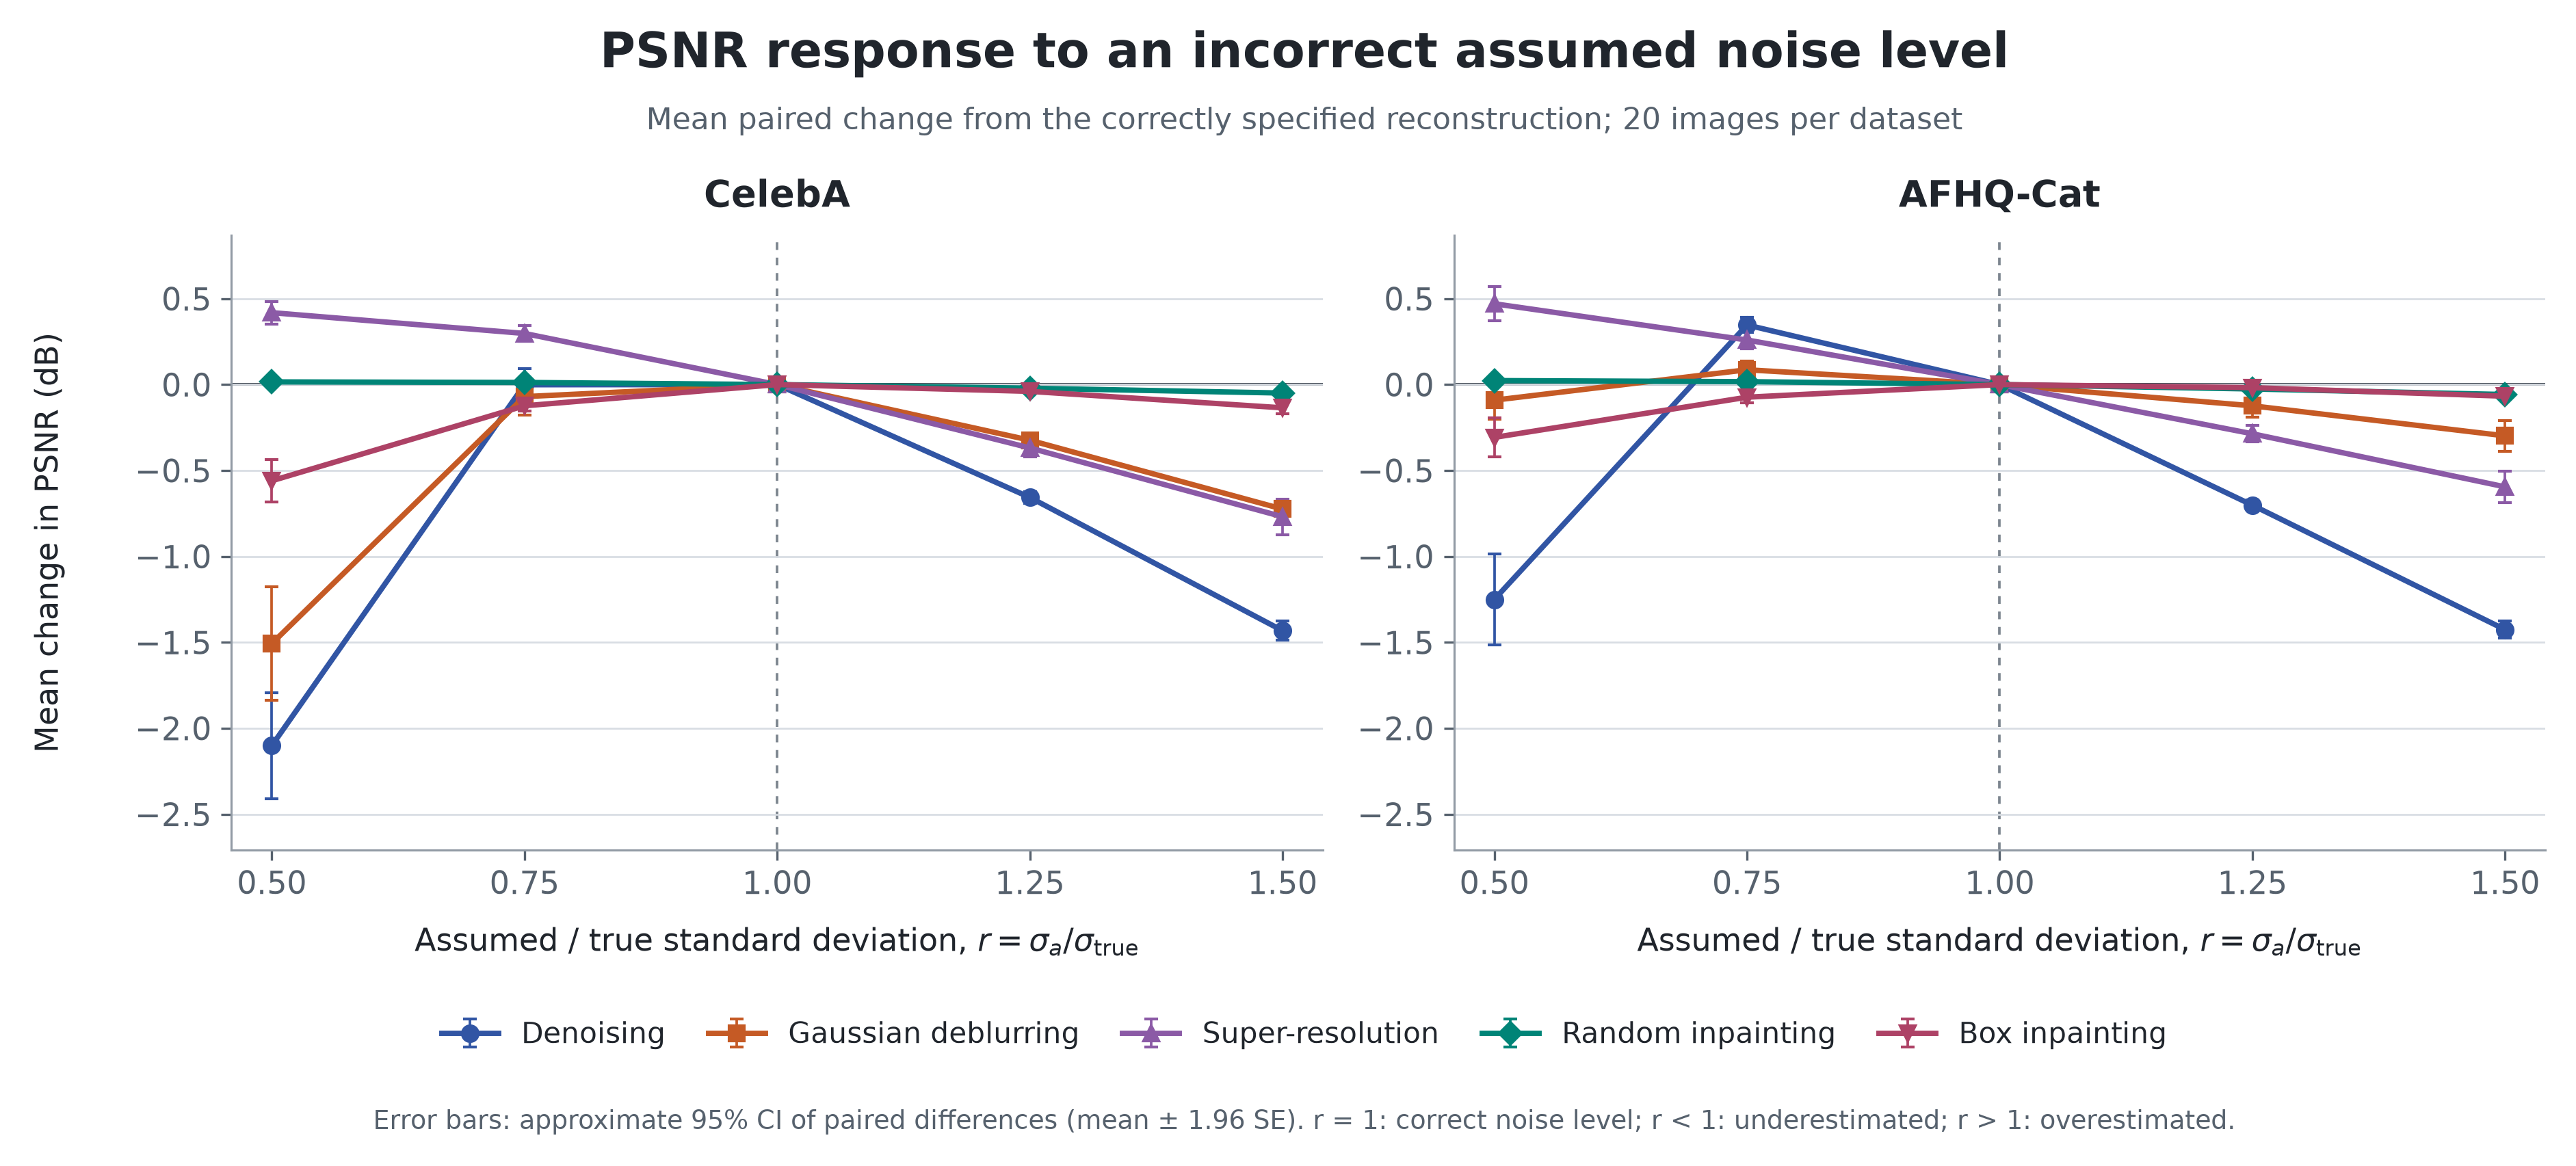
\includegraphics[width=\linewidth]{01_psnr_response.png}

\caption{
Paired PSNR changes for CelebA and AFHQ-Cat (20 images each).
Error bars are approximate 95\% intervals across images.
}

\label{fig:psnr}

\end{figure}


\begin{figure}[htbp]

\centering

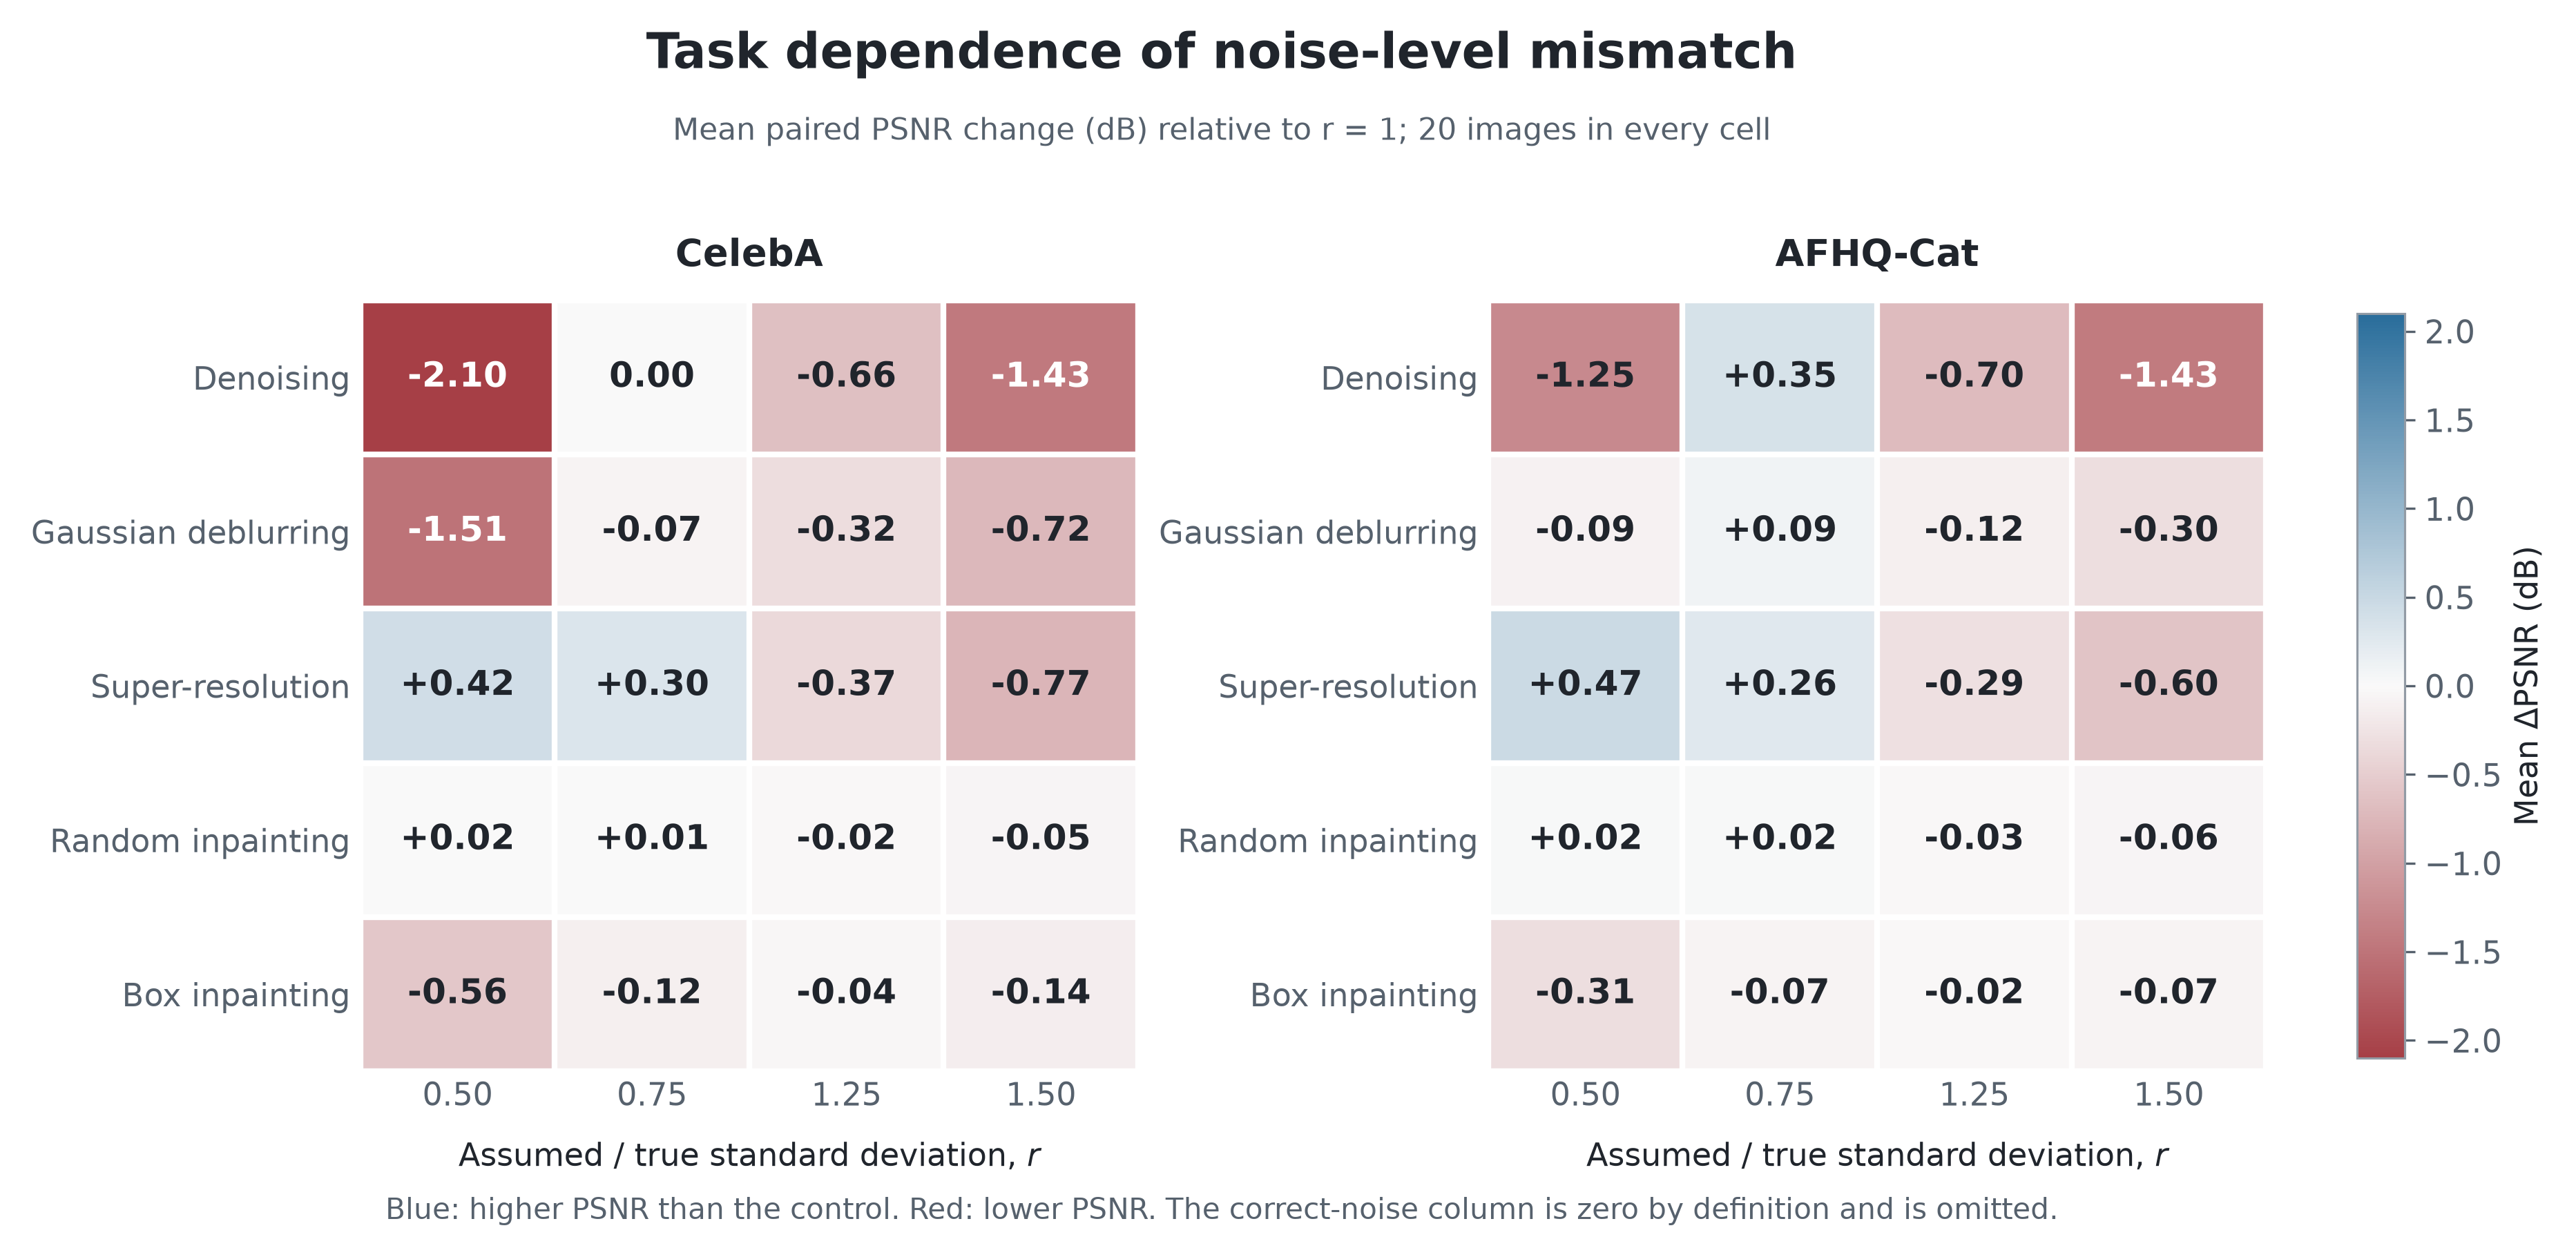
\includegraphics[width=\linewidth]{04_psnr_mismatch_map.png}

\caption{
Mean PSNR differences by inverse problem and assumed noise ratio.
Positive differences indicate improved fidelity compared with
the correct-noise control.
}

\label{fig:heatmap}

\end{figure}

To summarize sensitivity without cancellations between positive
and negative aggregate changes, define

\begin{equation}
    S_{d,k}
    =
    \frac14
    \sum_{r\ne1}
    \left|
        \overline{\Delta\mathrm{PSNR}}_{d,k}(r)
    \right|.
    \label{eq:sensitivity}
\end{equation}

CelebA and AFHQ-Cat denoising have the largest sensitivity values
($1.05$ dB and $0.93$ dB), whereas random inpainting has the
smallest ($0.02$ dB and $0.03$ dB).

This is the mean absolute change of the aggregate curve,
not the mean of individual-image absolute changes.


% ------------------------------------------------------------
% 5.3 SSIM AND LPIPS
% ------------------------------------------------------------

\subsection{Structural and perceptual agreement}

Figures~\ref{fig:ssim} and~\ref{fig:lpips} show that the three
metrics do not always agree.

Super-resolution at $r=0.5$ improves PSNR and SSIM and reduces
LPIPS in both datasets.

AFHQ-Cat denoising at $r=0.75$ also improves all three.

At $r=0.5$, however, AFHQ-Cat denoising has worse PSNR
and SSIM but better LPIPS, illustrating a perceptual--distortion trade-off.


\begin{figure}[htbp]

\centering

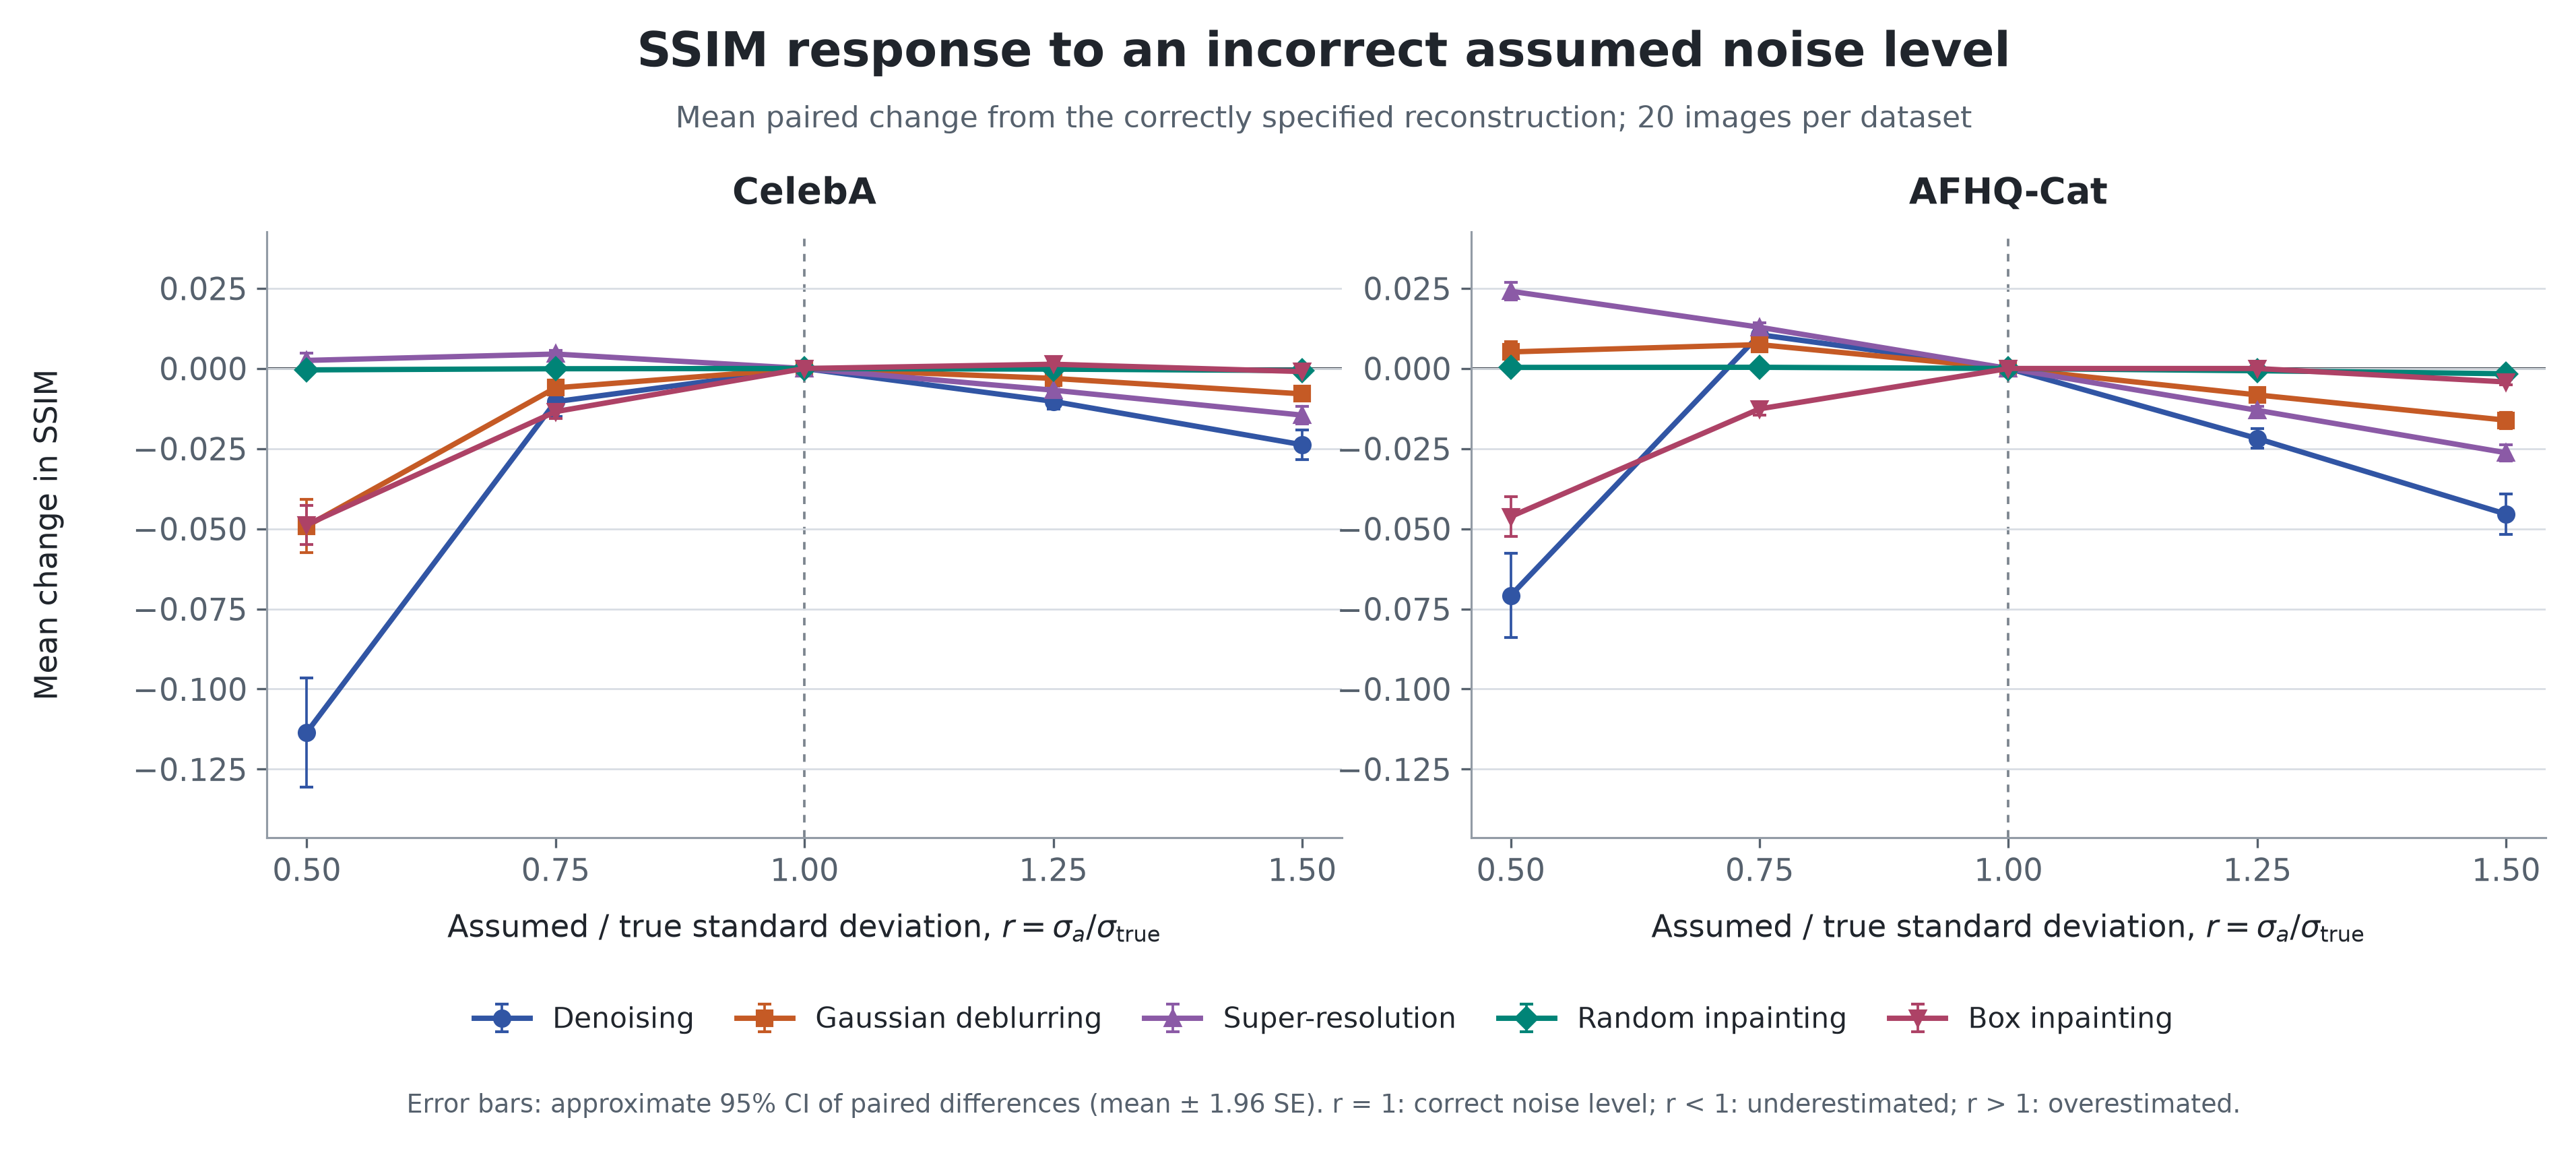
\includegraphics[width=\linewidth]{02_ssim_response.png}

\caption{
Paired SSIM differences.
Higher values indicate improved structural similarity.
}

\label{fig:ssim}

\end{figure}


\begin{figure}[htbp]

\centering

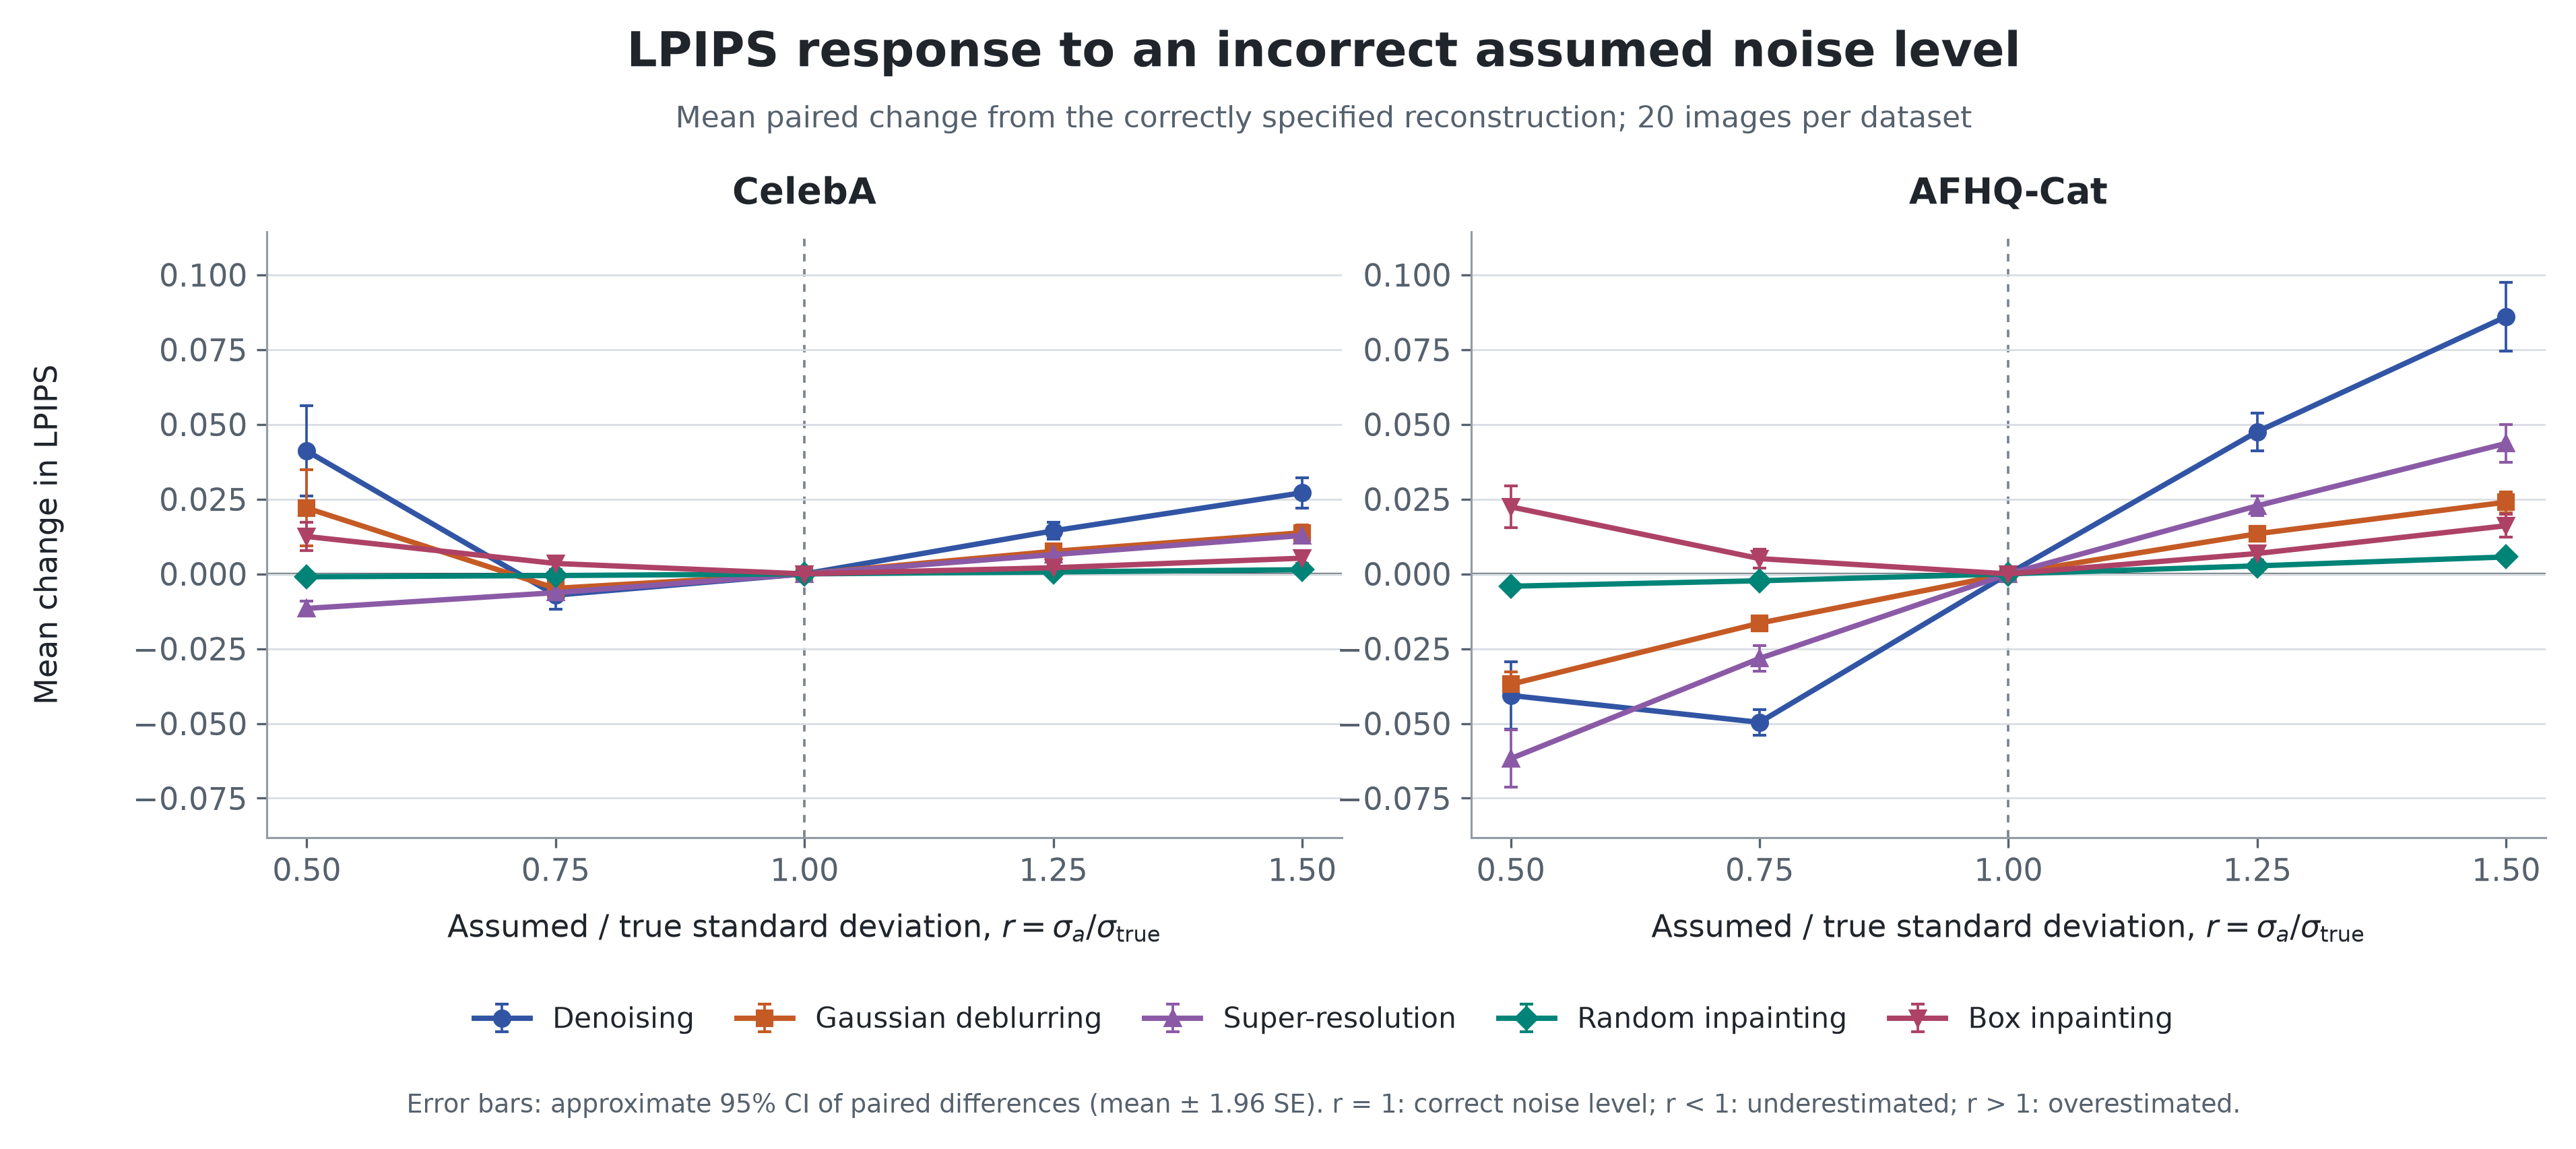
\includegraphics[width=\linewidth]{03_lpips_response.png}

\caption{
Paired LPIPS differences.
Lower values indicate improved perceptual similarity.
}

\label{fig:lpips}

\end{figure}


\begin{table}[htbp]

\centering
\footnotesize

\caption{
Selected paired metric changes.
PSNR and SSIM improve upward; LPIPS improves downward.
}

\label{tab:selected}

\resizebox{\textwidth}{!}{%

\begin{tabular}{llrrrr}

\toprule

Dataset & Task & $r$ & $\Delta$PSNR (dB) & $\Delta$SSIM & $\Delta$LPIPS\\

\midrule

CelebA & Denoising & 0.50 & -2.101 & -0.1135 & +0.0411\\
AFHQ-Cat & Denoising & 0.50 & -1.250 & -0.0708 & -0.0406\\
AFHQ-Cat & Denoising & 0.75 & +0.347 & +0.0106 & -0.0496\\
CelebA & Super-resolution & 0.50 & +0.419 & +0.0025 & -0.0115\\
AFHQ-Cat & Super-resolution & 0.50 & +0.470 & +0.0241 & -0.0618\\
CelebA & Random inpainting & 1.50 & -0.049 & -0.0006 & +0.0014\\
AFHQ-Cat & Random inpainting & 1.50 & -0.058 & -0.0016 & +0.0057\\

\bottomrule

\end{tabular}

}

\end{table}


% ------------------------------------------------------------
% 5.4 QUALITATIVE RESULTS
% ------------------------------------------------------------

\subsection{Qualitative reconstruction comparisons}

Figures~\ref{fig:celeba} and~\ref{fig:afhq} present fixed images
under all five noise assumptions and tasks.

Blue frames mark $r=1$; each task uses the same measurement
and source-noise draws across ratios.

The displayed \emph{measurement image} is $H^\top y$,
back-projected into image coordinates for visualization,
whereas FLOWER actually receives $y$.

The examples illustrate the aggregate behavior but do not substitute
for 20-image statistics.


\begin{figure}[htbp]

\centering

\makebox[\linewidth][c]{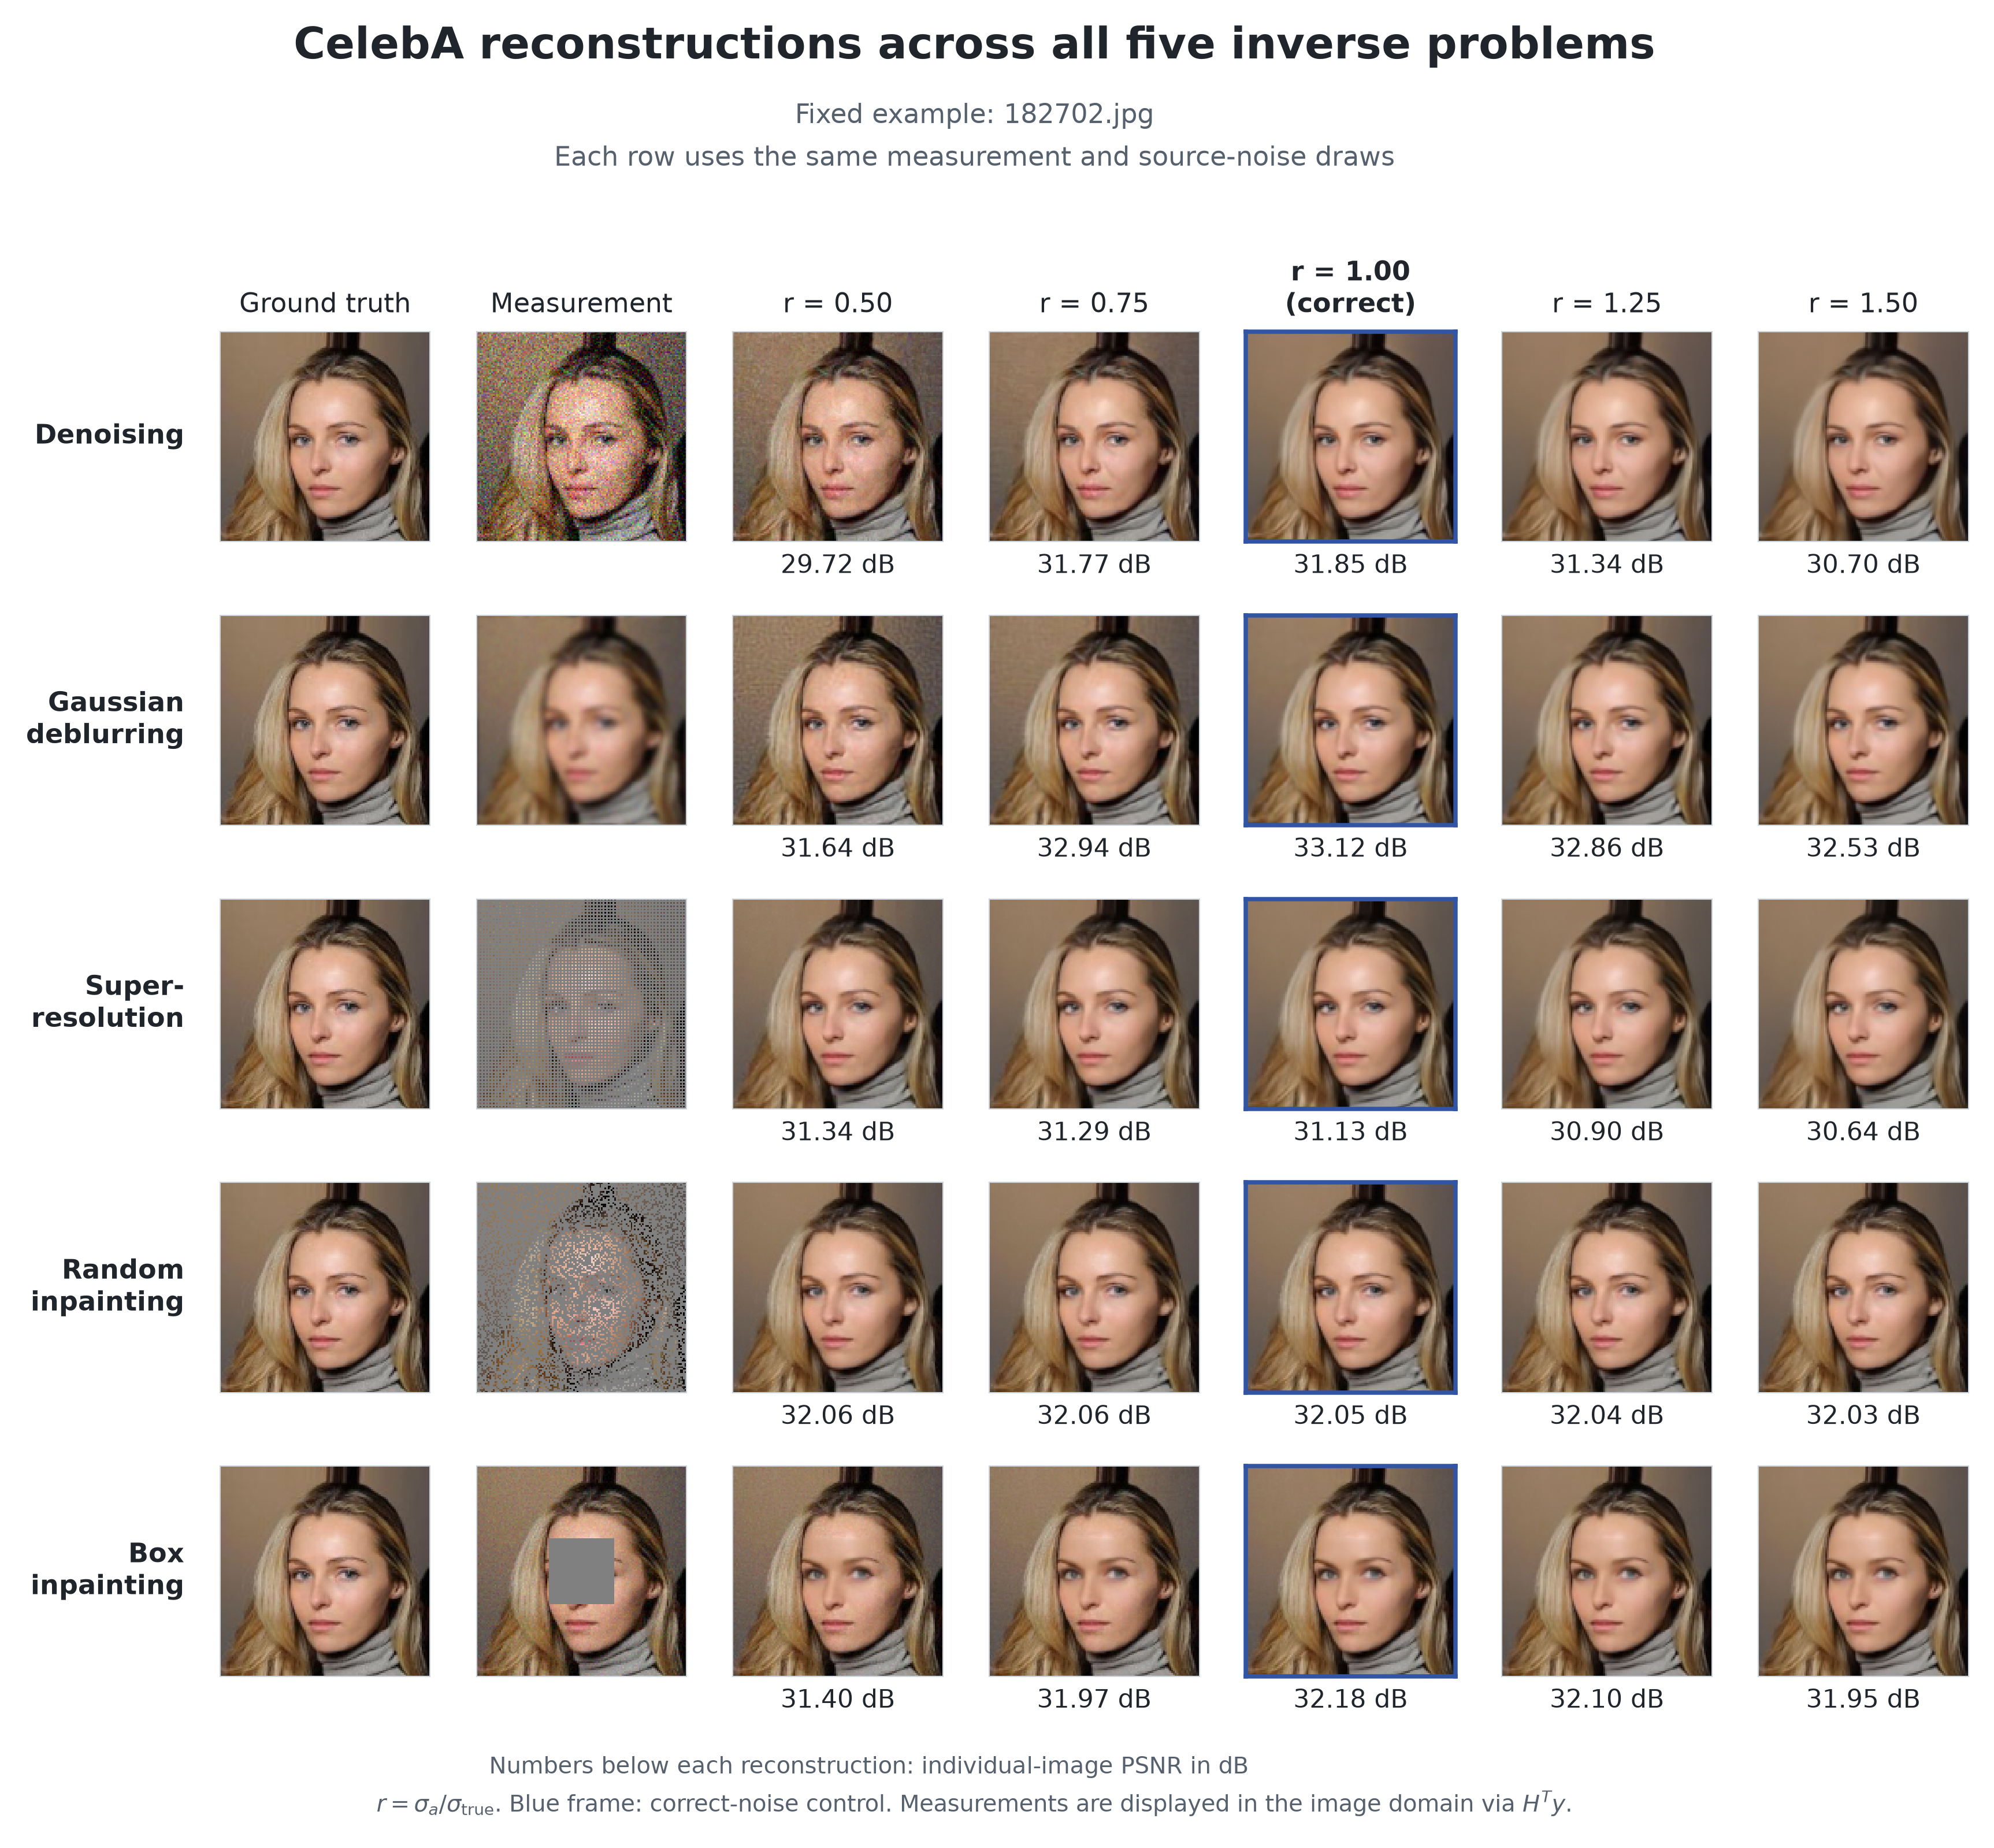
\includegraphics[width=1.12\linewidth,height=.73\textheight,keepaspectratio]{05_celeba_reconstructions.png}}

\caption{
CelebA qualitative comparison, image \texttt{182702.jpg}.
Values beneath reconstructions are single-image PSNR,
not dataset averages.
}

\label{fig:celeba}

\end{figure}



\begin{figure}[htbp]

\centering

\makebox[\linewidth][c]{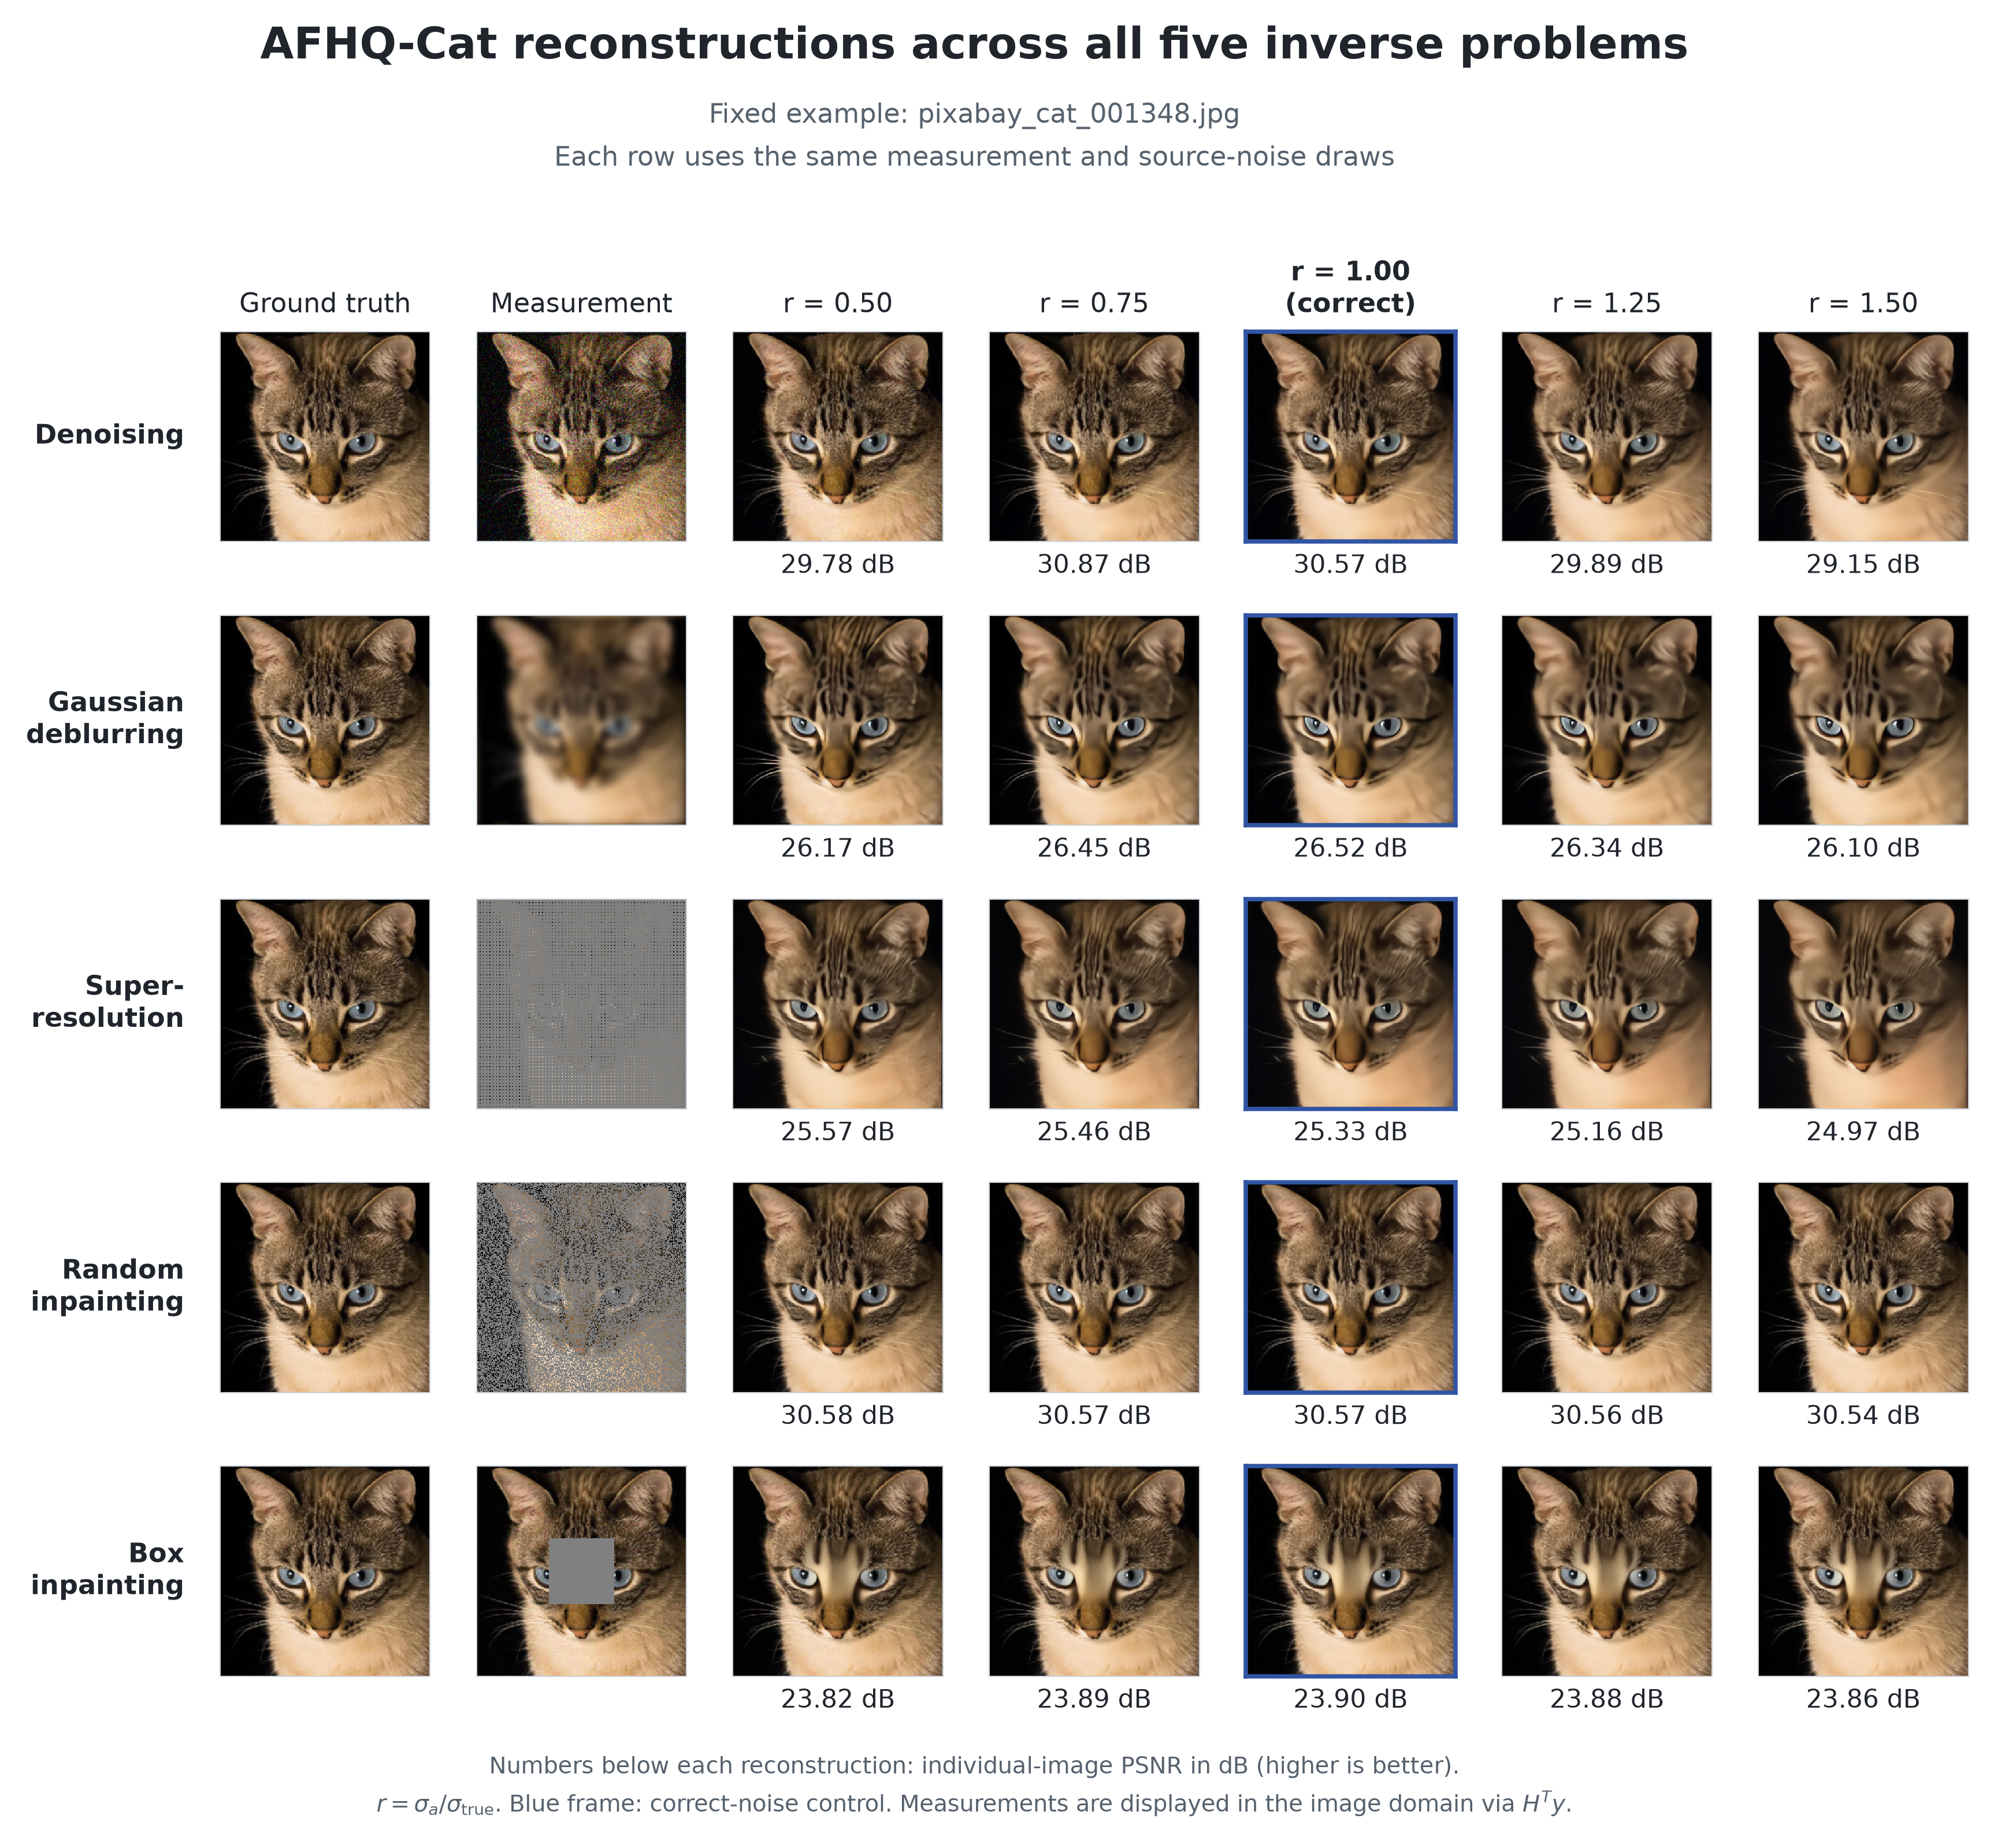
\includegraphics[width=1.12\linewidth,height=.73\textheight,keepaspectratio]{06_afhq_cat_reconstructions.png}}

\caption{
AFHQ-Cat qualitative comparison,
image \texttt{pixabay\_cat\_001348.jpg},
with the same column interpretation.
}

\label{fig:afhq}

\end{figure}



\FloatBarrier


% ------------------------------------------------------------
% 5.5 TRAJECTORY
% ------------------------------------------------------------

\subsection{What changes along the reconstruction trajectory}

Figure~\ref{fig:trajectory} follows a representative CelebA
denoising image, \texttt{182734.jpg}, selected near the median
image-level sensitivity in the most sensitive setting.

Early states contain strong source noise; changes between noise
assumptions become clearer as its coefficient shrinks.

Figure~\ref{fig:three} isolates the three steps at $t=0.75$:
the noise-scale assumption enters Step 2 directly but also
affects later Step 1 estimates indirectly through the changed trajectory.

Step 3 is a noisy state, not a clean endpoint estimate.


\begin{figure}[htbp]

\centering

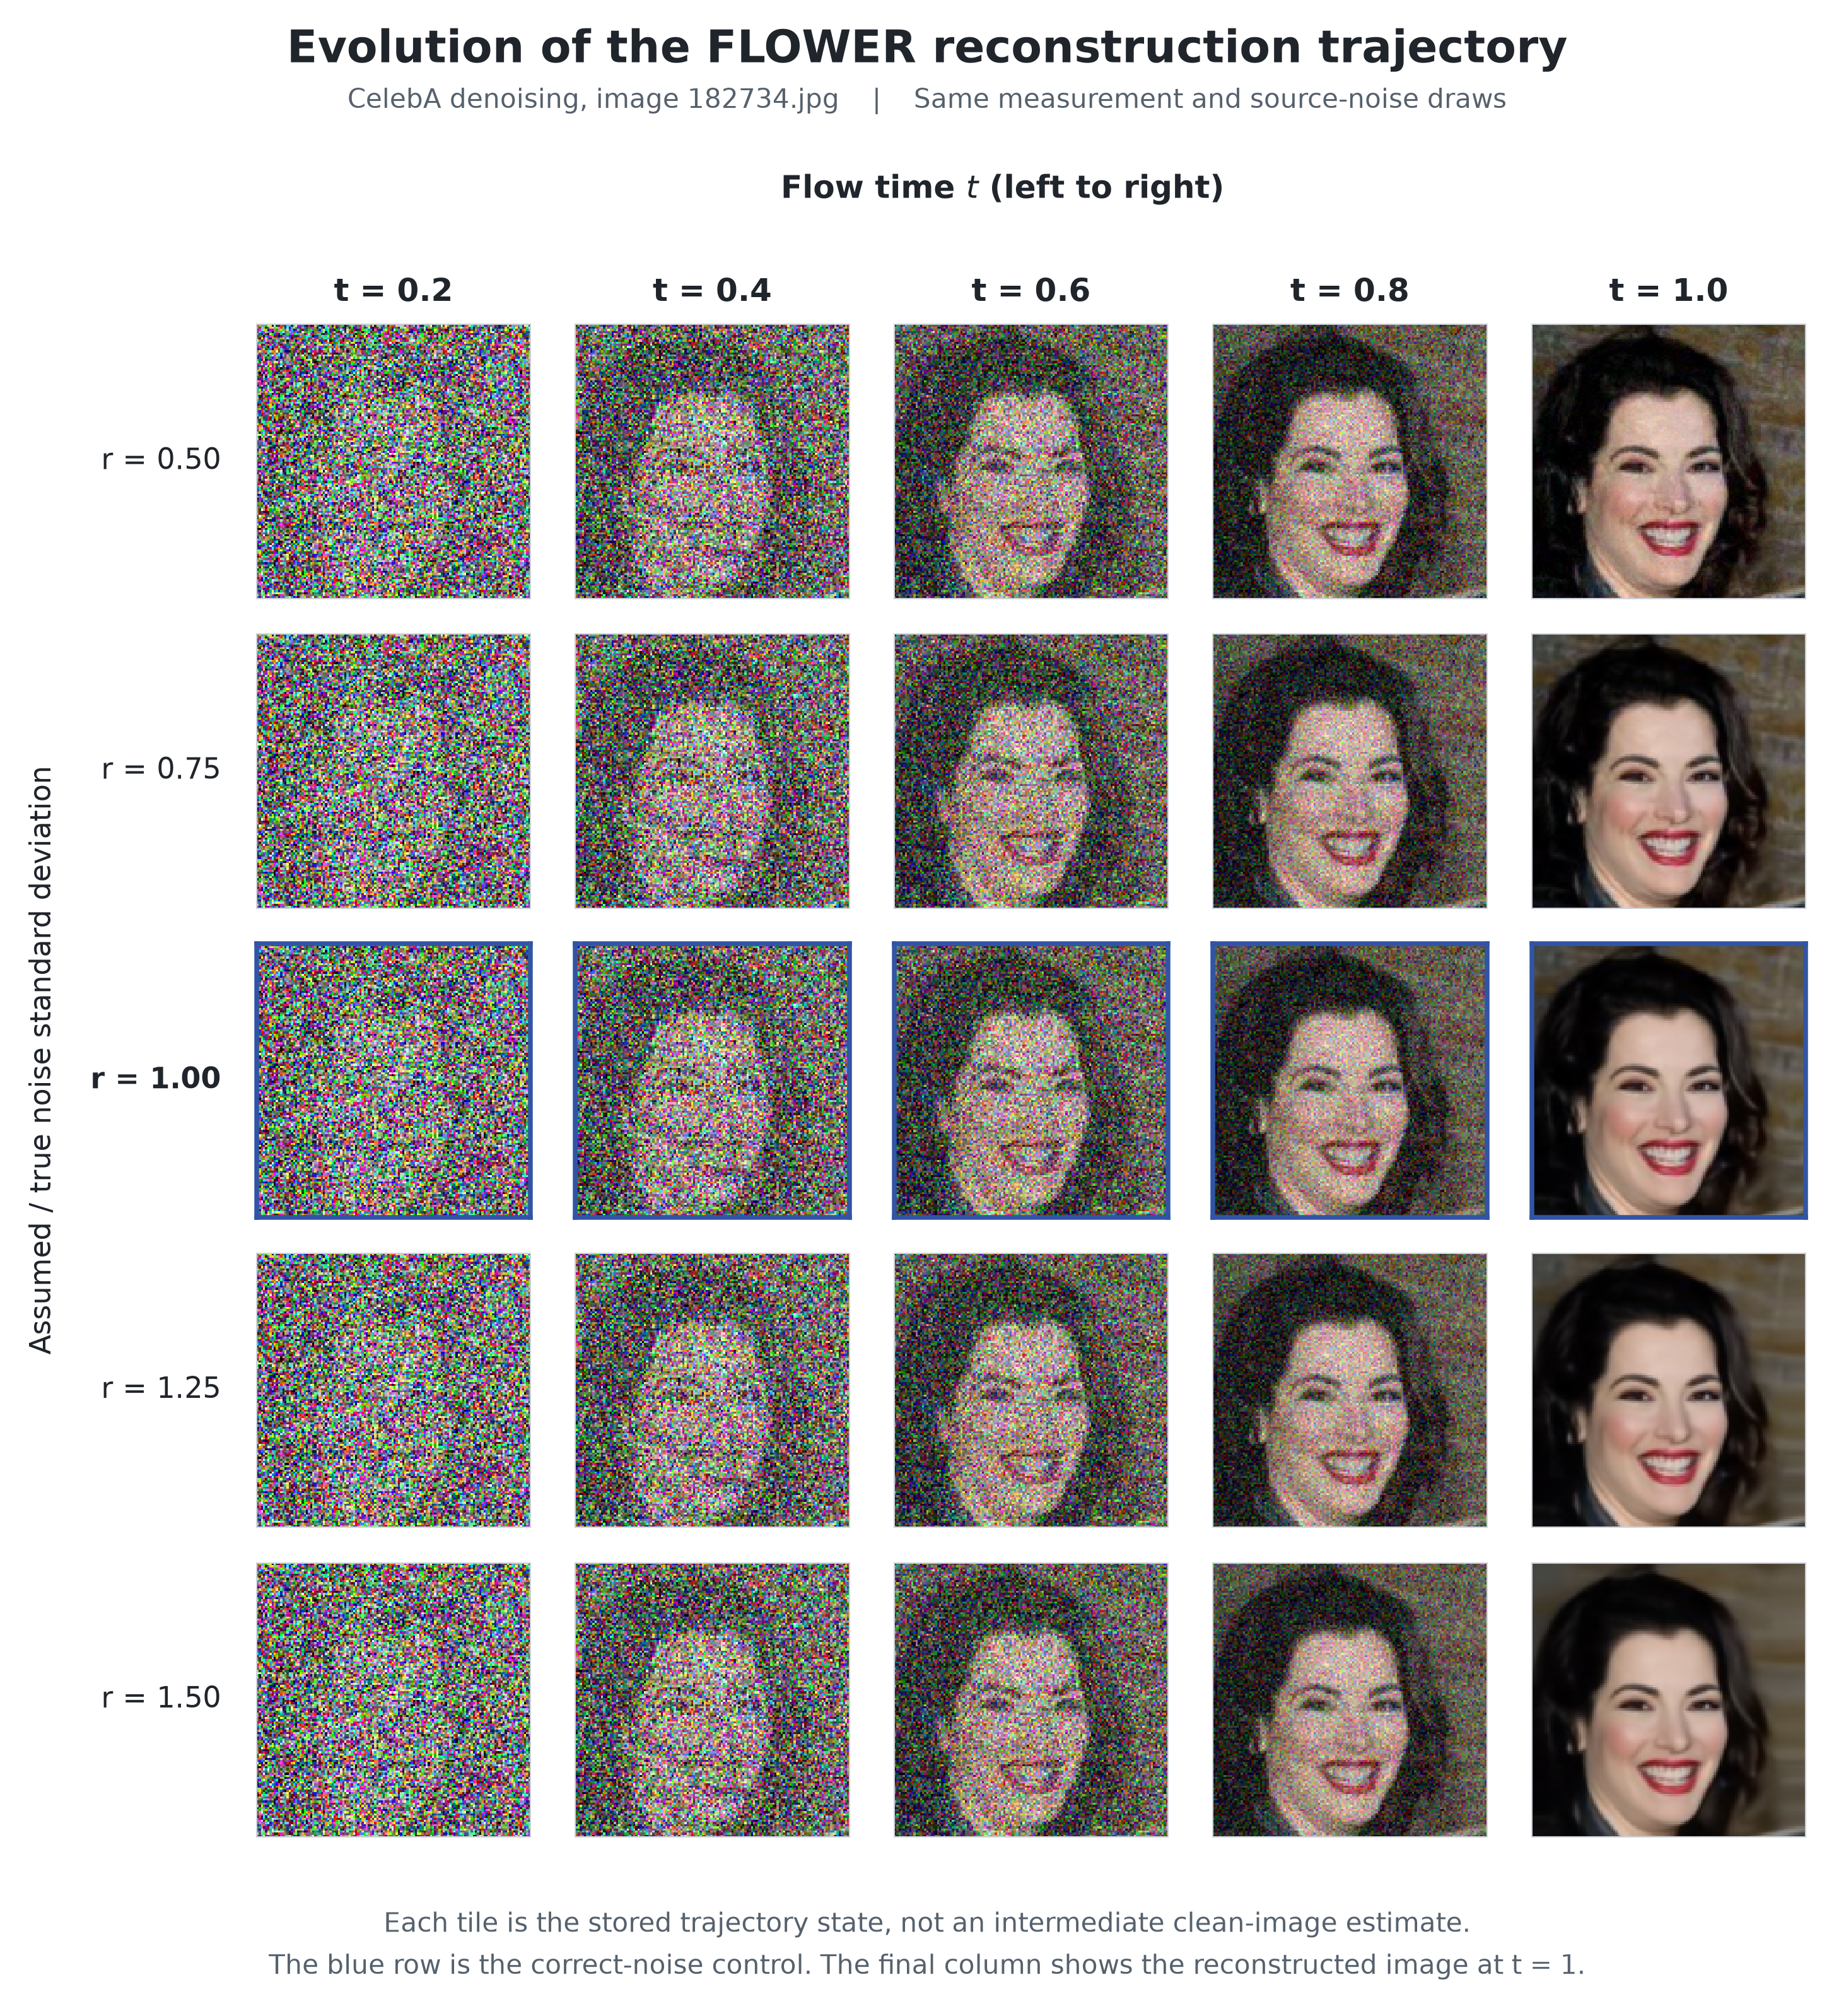
\includegraphics[width=.70\linewidth,height=.60\textheight,keepaspectratio]{07_reconstruction_trajectory.png}

\caption{
FLOWER trajectory states for CelebA denoising across
time and noise-scale ratios; the last column is the final reconstruction.
}

\label{fig:trajectory}

\end{figure}


\begin{figure}[htbp]

\centering

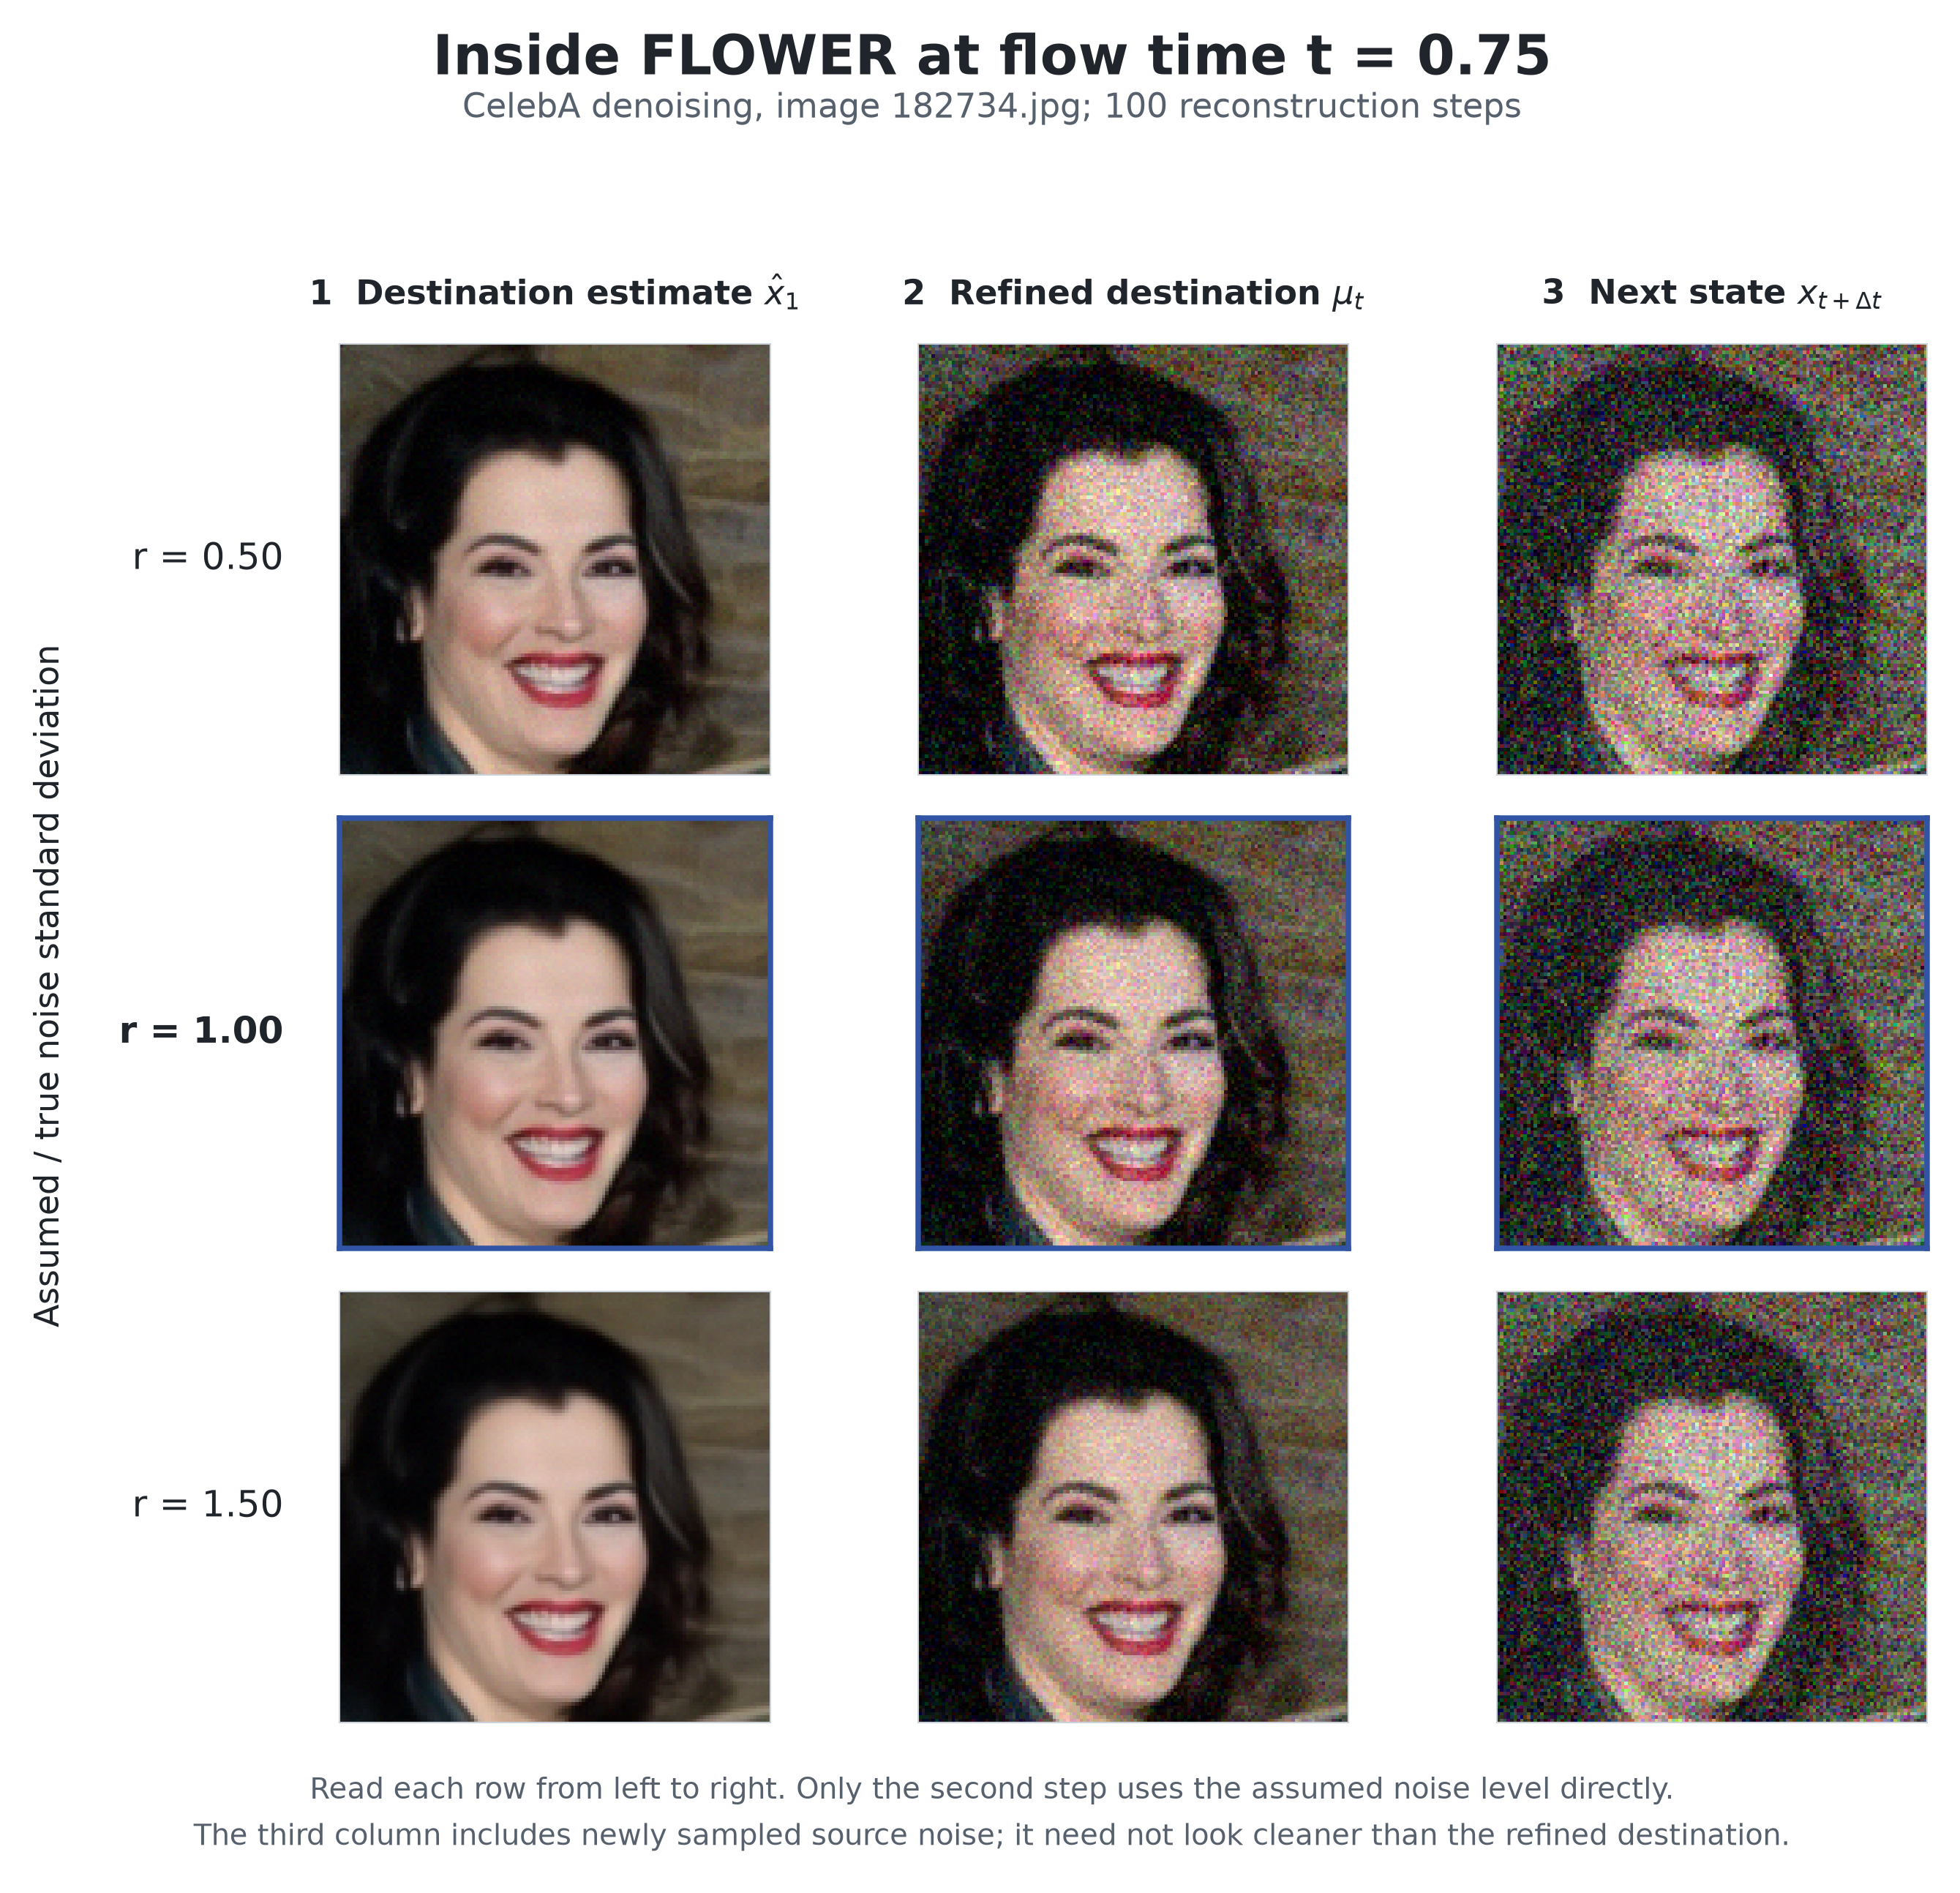
\includegraphics[width=.66\linewidth,height=.53\textheight,keepaspectratio]{08_internal_states_t075.png}

\caption{
Inside FLOWER at $t=0.75$:
clean destination estimate, measurement-refined destination,
and noisy next state.
}

\label{fig:three}

\end{figure}

\FloatBarrier


% ============================================================
% 6. DISCUSSION
% ============================================================

\section{Discussion}

% ------------------------------------------------------------
% 6.1
% ------------------------------------------------------------

\subsection{Operator dependence and calibration}

The study supports an operator-dependent, rather than universal,
conclusion.

Denoising can lose more than $2$ dB under severe noise
underestimation, while random inpainting is nearly invariant
within the tested range.

Equation~\eqref{eq:denoisingweight} explains the denoising response:
every pixel is directly involved in the measurement term,
so a wrong $\sa$ changes the refinement throughout the image.

For a binary inpainting mask, the data term directly constrains
only observed coordinates; unobserved coordinates are primarily
supplied by the learned destination.

Effects can still propagate to later iterations.

Random inpainting also uses the smallest true noise scale,
$\sx=0.01$.

Its apparent robustness cannot therefore be attributed to the
operator alone: task identity and true noise level co-vary.

The super-resolution gains under underestimation may compensate for
practical approximations in the reconstruction method, but the present
study does not isolate whether the cause lies in the learned prior,
the Gaussian endpoint approximation, discretization, or some other
implementation detail.


% ------------------------------------------------------------
% 6.2
% ------------------------------------------------------------

\subsection{Scope and limitations of the evidence}

Only 20 fixed images per dataset and one paired random sequence
per image--task pair are used.

The reported intervals therefore reflect selected image variability,
not independent solver-seed variability or guarantees across datasets.

I tested moderate positive scalar noise ratios rather than
unknown noise families or misspecified spatial covariance.

The ratio that maximizes a metric on this sample is descriptive,
not a validated noise-calibration rule.

Differences from published 100-image benchmark averages cannot be
conflated with within-image mismatch effects.


% ------------------------------------------------------------
% 6.3
% ------------------------------------------------------------

\subsection{Potential extension to nonlinear inverse problems}

The original FLOWER paper sketches a nonlinear measurement model
$y=h(x_1)+n$ with Gaussian noise.

The Gaussian endpoint approximation then produces

\begin{equation}
    \widetilde p(x_1\mid x_t,y)
    \propto
    \exp\left[
        -
        \frac{\|y-h(x_1)\|_2^2}{2\sa^2}
        -
        \frac{\|x_1-\widehat x_1\|_2^2}{2\nu_t^2}
    \right],
    \label{eq:nonlineardensity}
\end{equation}

which is generally non-Gaussian.

Its score is available:

\begin{equation}
    \nabla_{x_1}
    \log
    \widetilde p(x_1\mid x_t,y)
    =
    \sa^{-2}
    J_h(x_1)^\top
    \bigl(y-h(x_1)\bigr)
    -
    \nu_t^{-2}
    (x_1-\widehat x_1),
    \label{eq:nonlinearscore}
\end{equation}

where $J_h$ denotes the Jacobian of $h$.

The paper suggests replacing the closed-form Step 2 by an iterative
sampler, such as Langevin dynamics.

My linear experiments do not test robustness of this nonlinear extension.


% ============================================================
% 7. CONCLUSION
% ============================================================

\section{Conclusion}

FLOWER combines a pretrained flow-based destination estimate,
a Gaussian measurement refinement, and a source-noise time-progression
step.

The refinement exposes a precise mathematical mechanism by which
noise-scale misspecification changes reconstructions.

Its posterior-sampling motivation should be distinguished from the
practical OT and $\gamma=0$ restoration configuration.

In my paired study, severe underestimation harms denoising,
whereas super-resolution improves under underestimation on both datasets.

Random inpainting is nearly insensitive over the tested ratios,
and overestimation reduces average PSNR in every tested
dataset--task combination.

PSNR, SSIM, and LPIPS sometimes disagree;
consequently, no single metric fully characterizes robustness.

Correct physical noise calibration need not maximize every
image-quality metric of an approximate practical solver.


% ============================================================
% APPENDIX A - MATHEMATICS
% ============================================================

\appendix

\section{Additional Mathematical Details}

% ------------------------------------------------------------
% A.1
% ------------------------------------------------------------

\subsection{The Gaussian variance schedule}

Suppose

\begin{equation}
    X_0,X_1
    \sim
    \Normal(0,I)
\end{equation}

are independent and

\begin{equation}
    X_t=(1-t)X_0+tX_1.
\end{equation}

Then

\begin{equation}
    \Cov(X_t)
    =
    [t^2+(1-t)^2]I,
    \qquad
    \Cov(X_1,X_t)
    =
    tI.
\end{equation}

Gaussian conditioning gives

\begin{align}
    \Cov(X_1\mid X_t)
    &=
    I
    -
    tI
    \bigl(
        [t^2+(1-t)^2]I
    \bigr)^{-1}
    tI
    \\
    &=
    \left(
        1
        -
        \frac{t^2}{t^2+(1-t)^2}
    \right)I
    \\
    &=
    \frac{(1-t)^2}{t^2+(1-t)^2}I
    =
    \nu_t^2I.
\end{align}

This exact result for Gaussian endpoints motivates the schedule,
but does not establish isotropic endpoint uncertainty for natural images.


% ------------------------------------------------------------
% A.2
% ------------------------------------------------------------

\subsection{Sampling the refinement perturbation}

Let

\begin{equation}
    \epsilon_1\sim\Normal(0,I_d),
    \qquad
    \epsilon_2\sim\Normal(0,I_m)
\end{equation}

be independent.

Define

\begin{equation}
    \kappa_t
    =
    \Sigma_t
    \left(
        \nu_t^{-1}\epsilon_1
        +
        \sa^{-1}H^\top\epsilon_2
    \right).
\end{equation}

It is Gaussian with zero mean and covariance

\begin{align}
    \Cov(\kappa_t)
    &=
    \Sigma_t
    \Cov(
        \nu_t^{-1}\epsilon_1
        +
        \sa^{-1}H^\top\epsilon_2
    )
    \Sigma_t^\top
    \\
    &=
    \Sigma_t
    (
        \nu_t^{-2}I
        +
        \sa^{-2}H^\top H
    )
    \Sigma_t^\top
    \\
    &=
    \Sigma_t
    \Sigma_t^{-1}
    \Sigma_t
    =
    \Sigma_t.
\end{align}

Thus

\begin{equation}
    \kappa_t\sim\Normal(0,\Sigma_t)
\end{equation}

without explicitly computing $\Sigma_t^{1/2}$.

When $\gamma=0$, this perturbation is omitted.


% ------------------------------------------------------------
% A.3
% ------------------------------------------------------------

\subsection{Known non-isotropic Gaussian noise}

For general known covariance $R_n\succ0$,

\begin{equation}
    n\sim\Normal(0,R_n),
\end{equation}

the data-fidelity term is

\begin{equation}
    F_y(x)
    =
    \frac12
    (y-Hx)^\top
    R_n^{-1}
    (y-Hx).
\end{equation}

The Gaussian posterior-refinement formulas become

\begin{align}
    \Sigma_t
    &=
    (
        \nu_t^{-2}I
        +
        H^\top R_n^{-1}H
    )^{-1},
    \\
    \mu_t
    &=
    \Sigma_t
    (
        \nu_t^{-2}\widehat x_1
        +
        H^\top R_n^{-1}y
    ).
\end{align}

This is the covariance-aware extension described in the original paper.

My experiment does not vary the covariance structure $R_n$
independently of the scalar noise scale.


% ============================================================
% APPENDIX B - REPRODUCIBILITY
% ============================================================

\section{Evaluation and Reproducibility Details}
\label{app:evaluation}

Numerical results reside in
\texttt{artifacts/experiments/main/}.

\texttt{metrics.csv} contains the 1,000 image-level rows;
\texttt{metrics\_with\_deltas.csv} contains paired differences;
and \texttt{summary.csv} contains the 50 dataset--task--ratio aggregates.

\texttt{run\_metadata.json} stores the experimental settings and seeds,
while selected filenames are stored under \texttt{data\_splits/}.

Selected qualitative and trajectory PNGs are provided,
but not a PNG for every numerical reconstruction.

PSNR and SSIM are computed on clipped $[0,1]$ images.

PSNR uses \texttt{skimage} with data range 1 and SSIM uses the
PyTorch-Ignite implementation.

LPIPS uses AlexNet and reproduces the public-code convention:
postprocessed images are mapped to $[-1,1]$ and the call sets
\texttt{normalize=True}.

This differs from the usual LPIPS convention,
but it is identical across all tested ratios.

The stored CSV metrics are the numerical source of truth;
the displayed PNGs underwent quantization.

The uncertainty intervals reproduce the original stored
normal-approximation summaries.


% ============================================================
% APPENDIX C - COMPLETE RESULTS
% ============================================================

\section{Complete Numerical Results}

Each entry in Tables~\ref{tab:allceleba} and~\ref{tab:allafhq}
is averaged over 20 fixed images.

The $r=1$ rows define the correctly specified control;
$\Delta\mathrm{PSNR}$ is paired with the same image's control.


% ------------------------------------------------------------
% CELEBA
% ------------------------------------------------------------

\begin{longtable}{lrrrrr}

\caption{
Complete CelebA results (20 fixed images per row).
}
\label{tab:allceleba}
\\

\toprule
Task & $r$ & PSNR & SSIM & LPIPS & $\Delta$PSNR\\
\midrule
\endfirsthead

\toprule
Task & $r$ & PSNR & SSIM & LPIPS & $\Delta$PSNR\\
\midrule
\endhead

Denoising & 0.50 & 30.12 & 0.803 & 0.072 & -2.101\\
& 0.75 & 32.22 & 0.906 & 0.024 & -0.001\\
& 1.00 & 32.22 & 0.917 & 0.031 & 0.000\\
& 1.25 & 31.57 & 0.906 & 0.045 & -0.657\\
& 1.50 & 30.79 & 0.893 & 0.058 & -1.432\\

\midrule

Deblurring & 0.50 & 33.24 & 0.898 & 0.047 & -1.507\\
& 0.75 & 34.67 & 0.941 & 0.020 & -0.070\\
& 1.00 & 34.74 & 0.947 & 0.025 & 0.000\\
& 1.25 & 34.42 & 0.944 & 0.032 & -0.324\\
& 1.50 & 34.02 & 0.939 & 0.039 & -0.724\\

\midrule

Super-resolution & 0.50 & 32.55 & 0.926 & 0.021 & +0.419\\
& 0.75 & 32.43 & 0.928 & 0.027 & +0.297\\
& 1.00 & 32.14 & 0.923 & 0.033 & 0.000\\
& 1.25 & 31.77 & 0.917 & 0.039 & -0.369\\
& 1.50 & 31.37 & 0.909 & 0.046 & -0.769\\

\midrule

Random inpainting & 0.50 & 32.66 & 0.943 & 0.016 & +0.016\\
& 0.75 & 32.66 & 0.943 & 0.016 & +0.012\\
& 1.00 & 32.65 & 0.943 & 0.017 & 0.000\\
& 1.25 & 32.63 & 0.943 & 0.018 & -0.021\\
& 1.50 & 32.60 & 0.942 & 0.018 & -0.049\\

\midrule

Box inpainting & 0.50 & 29.98 & 0.897 & 0.033 & -0.560\\
& 0.75 & 30.41 & 0.932 & 0.024 & -0.124\\
& 1.00 & 30.54 & 0.946 & 0.021 & 0.000\\
& 1.25 & 30.50 & 0.947 & 0.023 & -0.040\\
& 1.50 & 30.40 & 0.945 & 0.026 & -0.135\\

\bottomrule

\end{longtable}


% ------------------------------------------------------------
% AFHQ-CAT
% ------------------------------------------------------------

\begin{longtable}{lrrrrr}

\caption{
Complete AFHQ-Cat results (20 fixed images per row).
}
\label{tab:allafhq}
\\

\toprule
Task & $r$ & PSNR & SSIM & LPIPS & $\Delta$PSNR\\
\midrule
\endfirsthead

\toprule
Task & $r$ & PSNR & SSIM & LPIPS & $\Delta$PSNR\\
\midrule
\endhead

Denoising & 0.50 & 30.06 & 0.805 & 0.068 & -1.250\\
& 0.75 & 31.65 & 0.886 & 0.059 & +0.347\\
& 1.00 & 31.31 & 0.875 & 0.109 & 0.000\\
& 1.25 & 30.61 & 0.854 & 0.157 & -0.702\\
& 1.50 & 29.88 & 0.830 & 0.195 & -1.426\\

\midrule

Deblurring & 0.50 & 27.36 & 0.756 & 0.260 & -0.091\\
& 0.75 & 27.54 & 0.759 & 0.280 & +0.086\\
& 1.00 & 27.45 & 0.751 & 0.297 & 0.000\\
& 1.25 & 27.33 & 0.743 & 0.310 & -0.123\\
& 1.50 & 27.15 & 0.735 & 0.321 & -0.298\\

\midrule

Super-resolution & 0.50 & 26.62 & 0.756 & 0.225 & +0.470\\
& 0.75 & 26.41 & 0.745 & 0.259 & +0.259\\
& 1.00 & 26.15 & 0.732 & 0.287 & 0.000\\
& 1.25 & 25.86 & 0.719 & 0.310 & -0.286\\
& 1.50 & 25.56 & 0.706 & 0.331 & -0.595\\

\midrule

Random inpainting & 0.50 & 32.17 & 0.912 & 0.042 & +0.023\\
& 0.75 & 32.17 & 0.912 & 0.043 & +0.017\\
& 1.00 & 32.15 & 0.912 & 0.046 & 0.000\\
& 1.25 & 32.12 & 0.911 & 0.048 & -0.026\\
& 1.50 & 32.09 & 0.910 & 0.051 & -0.058\\

\midrule

Box inpainting & 0.50 & 26.39 & 0.871 & 0.084 & -0.307\\
& 0.75 & 26.62 & 0.905 & 0.066 & -0.074\\
& 1.00 & 26.70 & 0.917 & 0.061 & 0.000\\
& 1.25 & 26.68 & 0.917 & 0.068 & -0.018\\
& 1.50 & 26.63 & 0.913 & 0.077 & -0.068\\

\bottomrule

\end{longtable}


% ============================================================
% APPENDIX D - EARLIER INTERNAL STATES
% ============================================================

\section{Earlier Internal States}

Figures~\ref{fig:early025} and~\ref{fig:early050}
repeat the three-step diagnostic at earlier flow times,
using the same source-noise and measurement controls
as in Figure~\ref{fig:three}.


\begin{figure}[htbp]

\centering

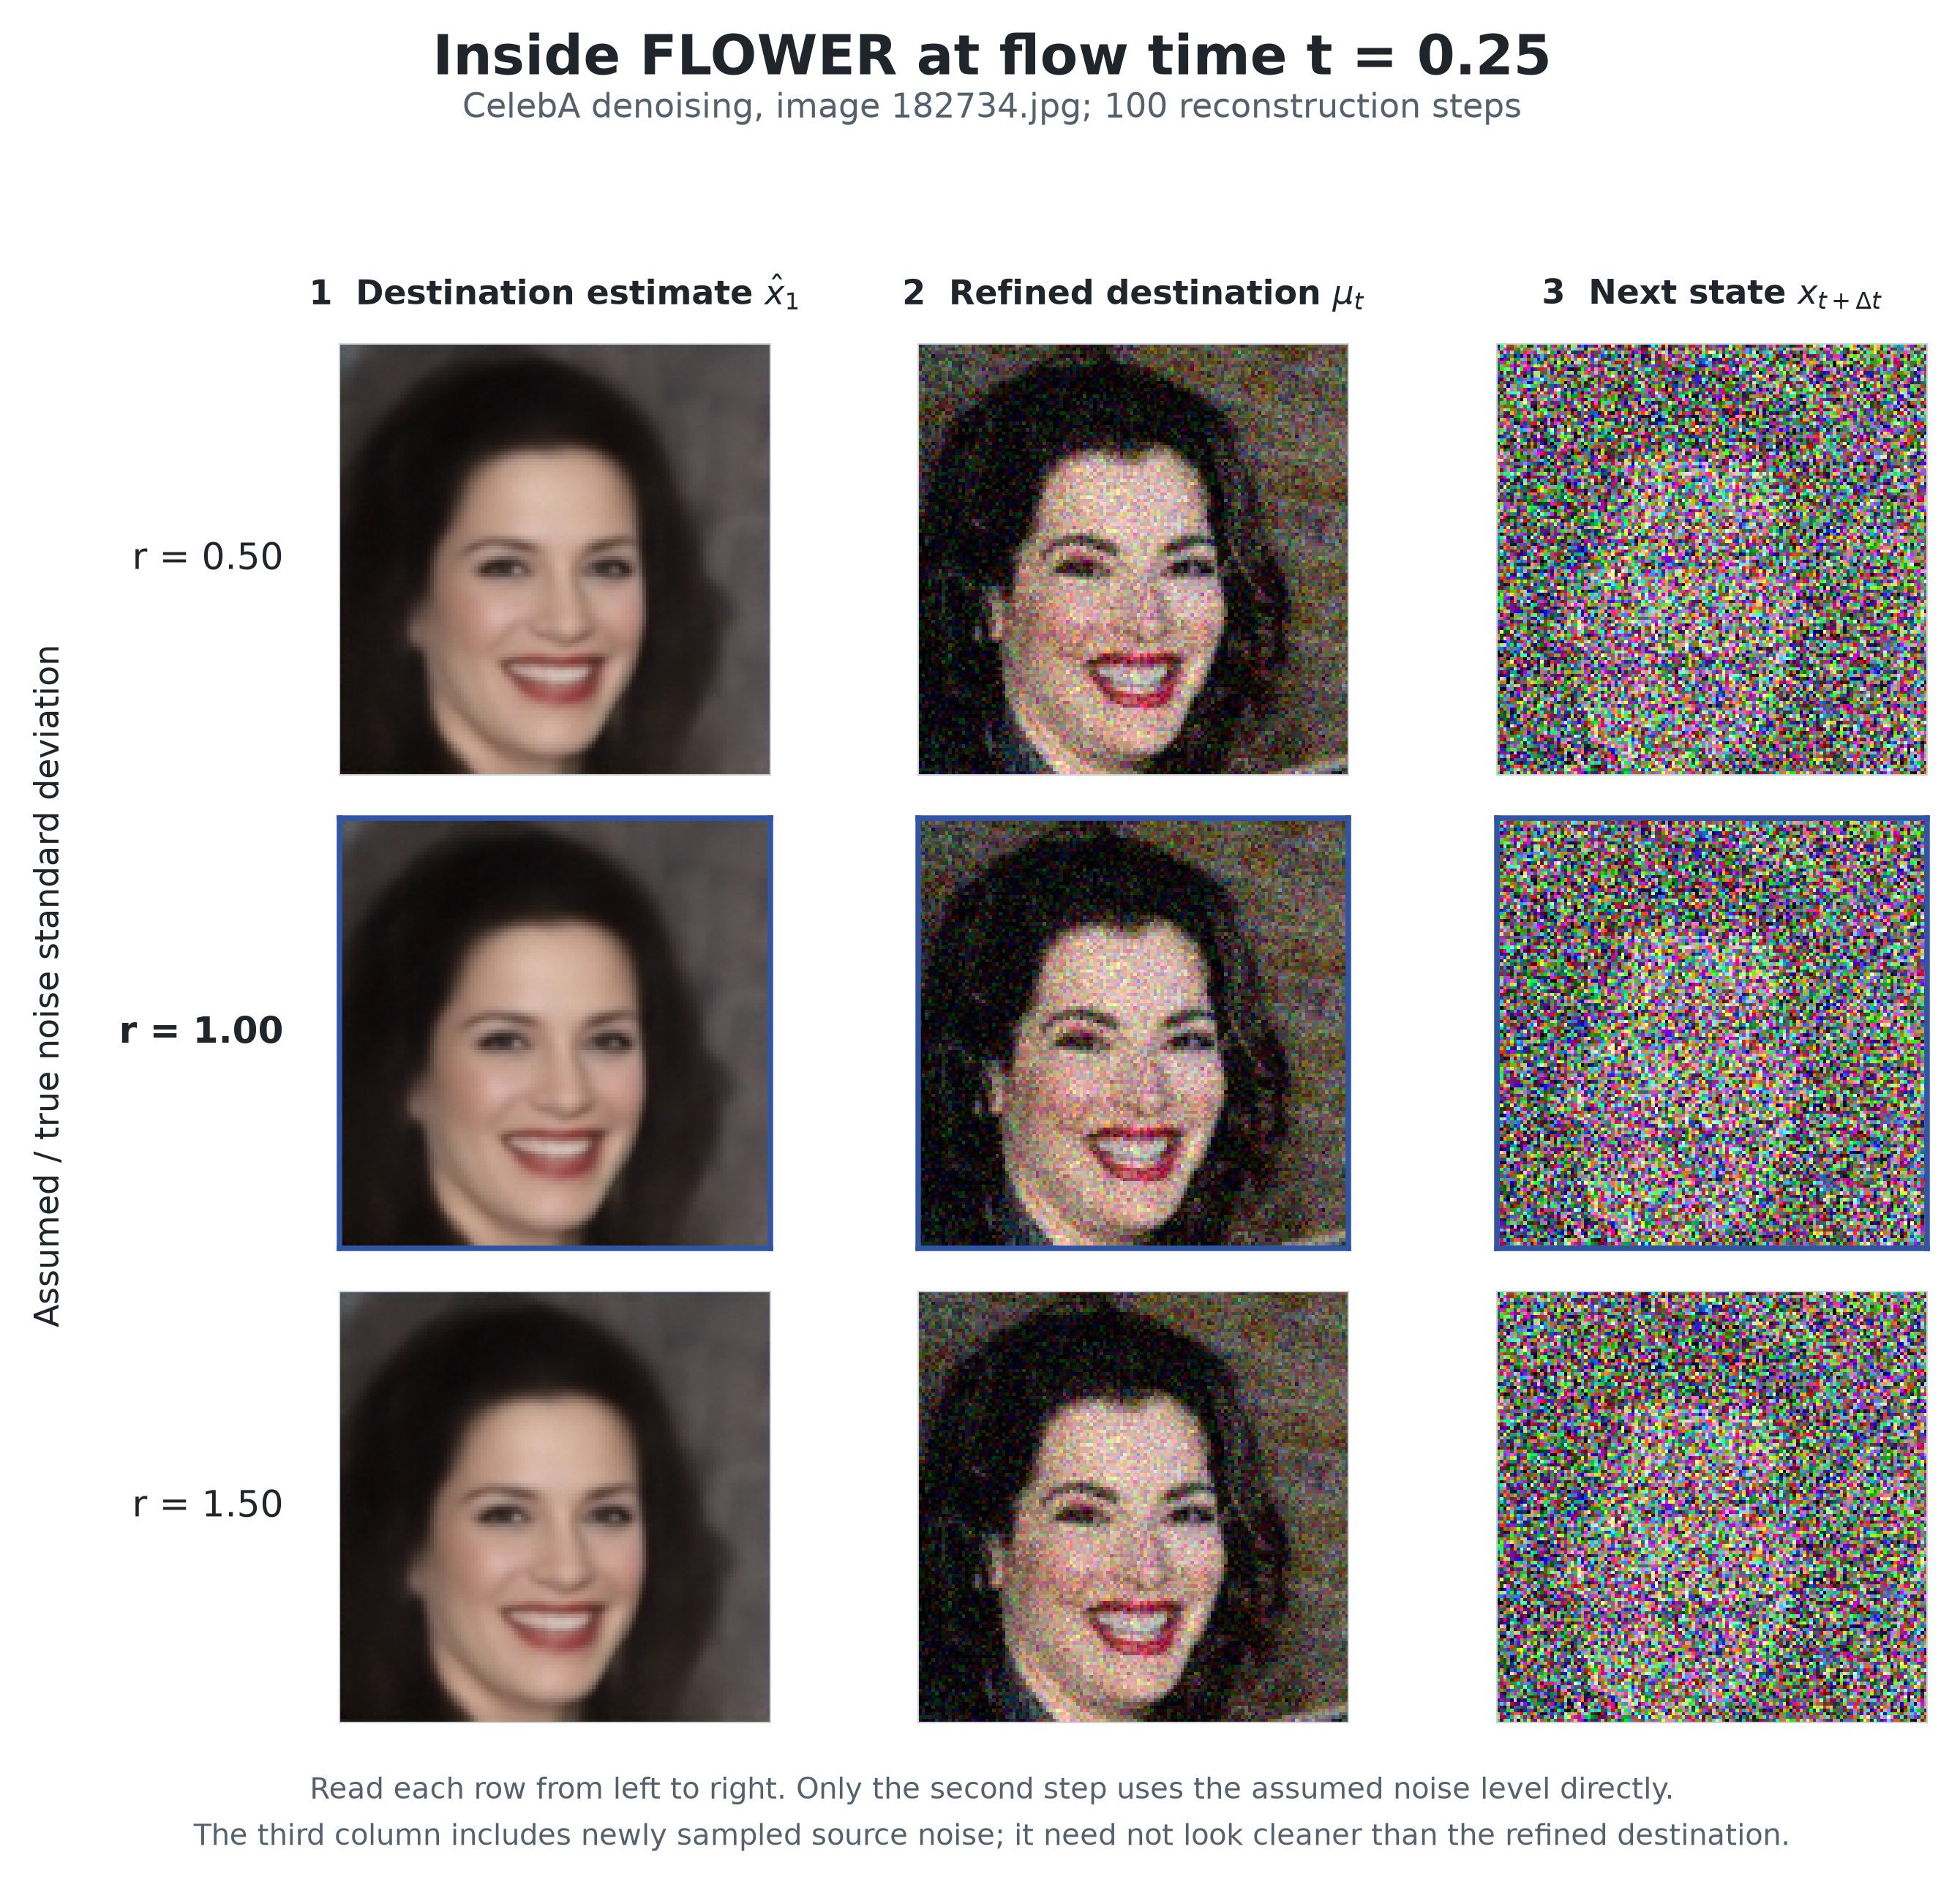
\includegraphics[width=.68\linewidth,height=.42\textheight,keepaspectratio]{09_internal_states_t025.png}

\caption{
Three internal FLOWER steps at $t=0.25$.
}

\label{fig:early025}

\end{figure}


\begin{figure}[htbp]

\centering

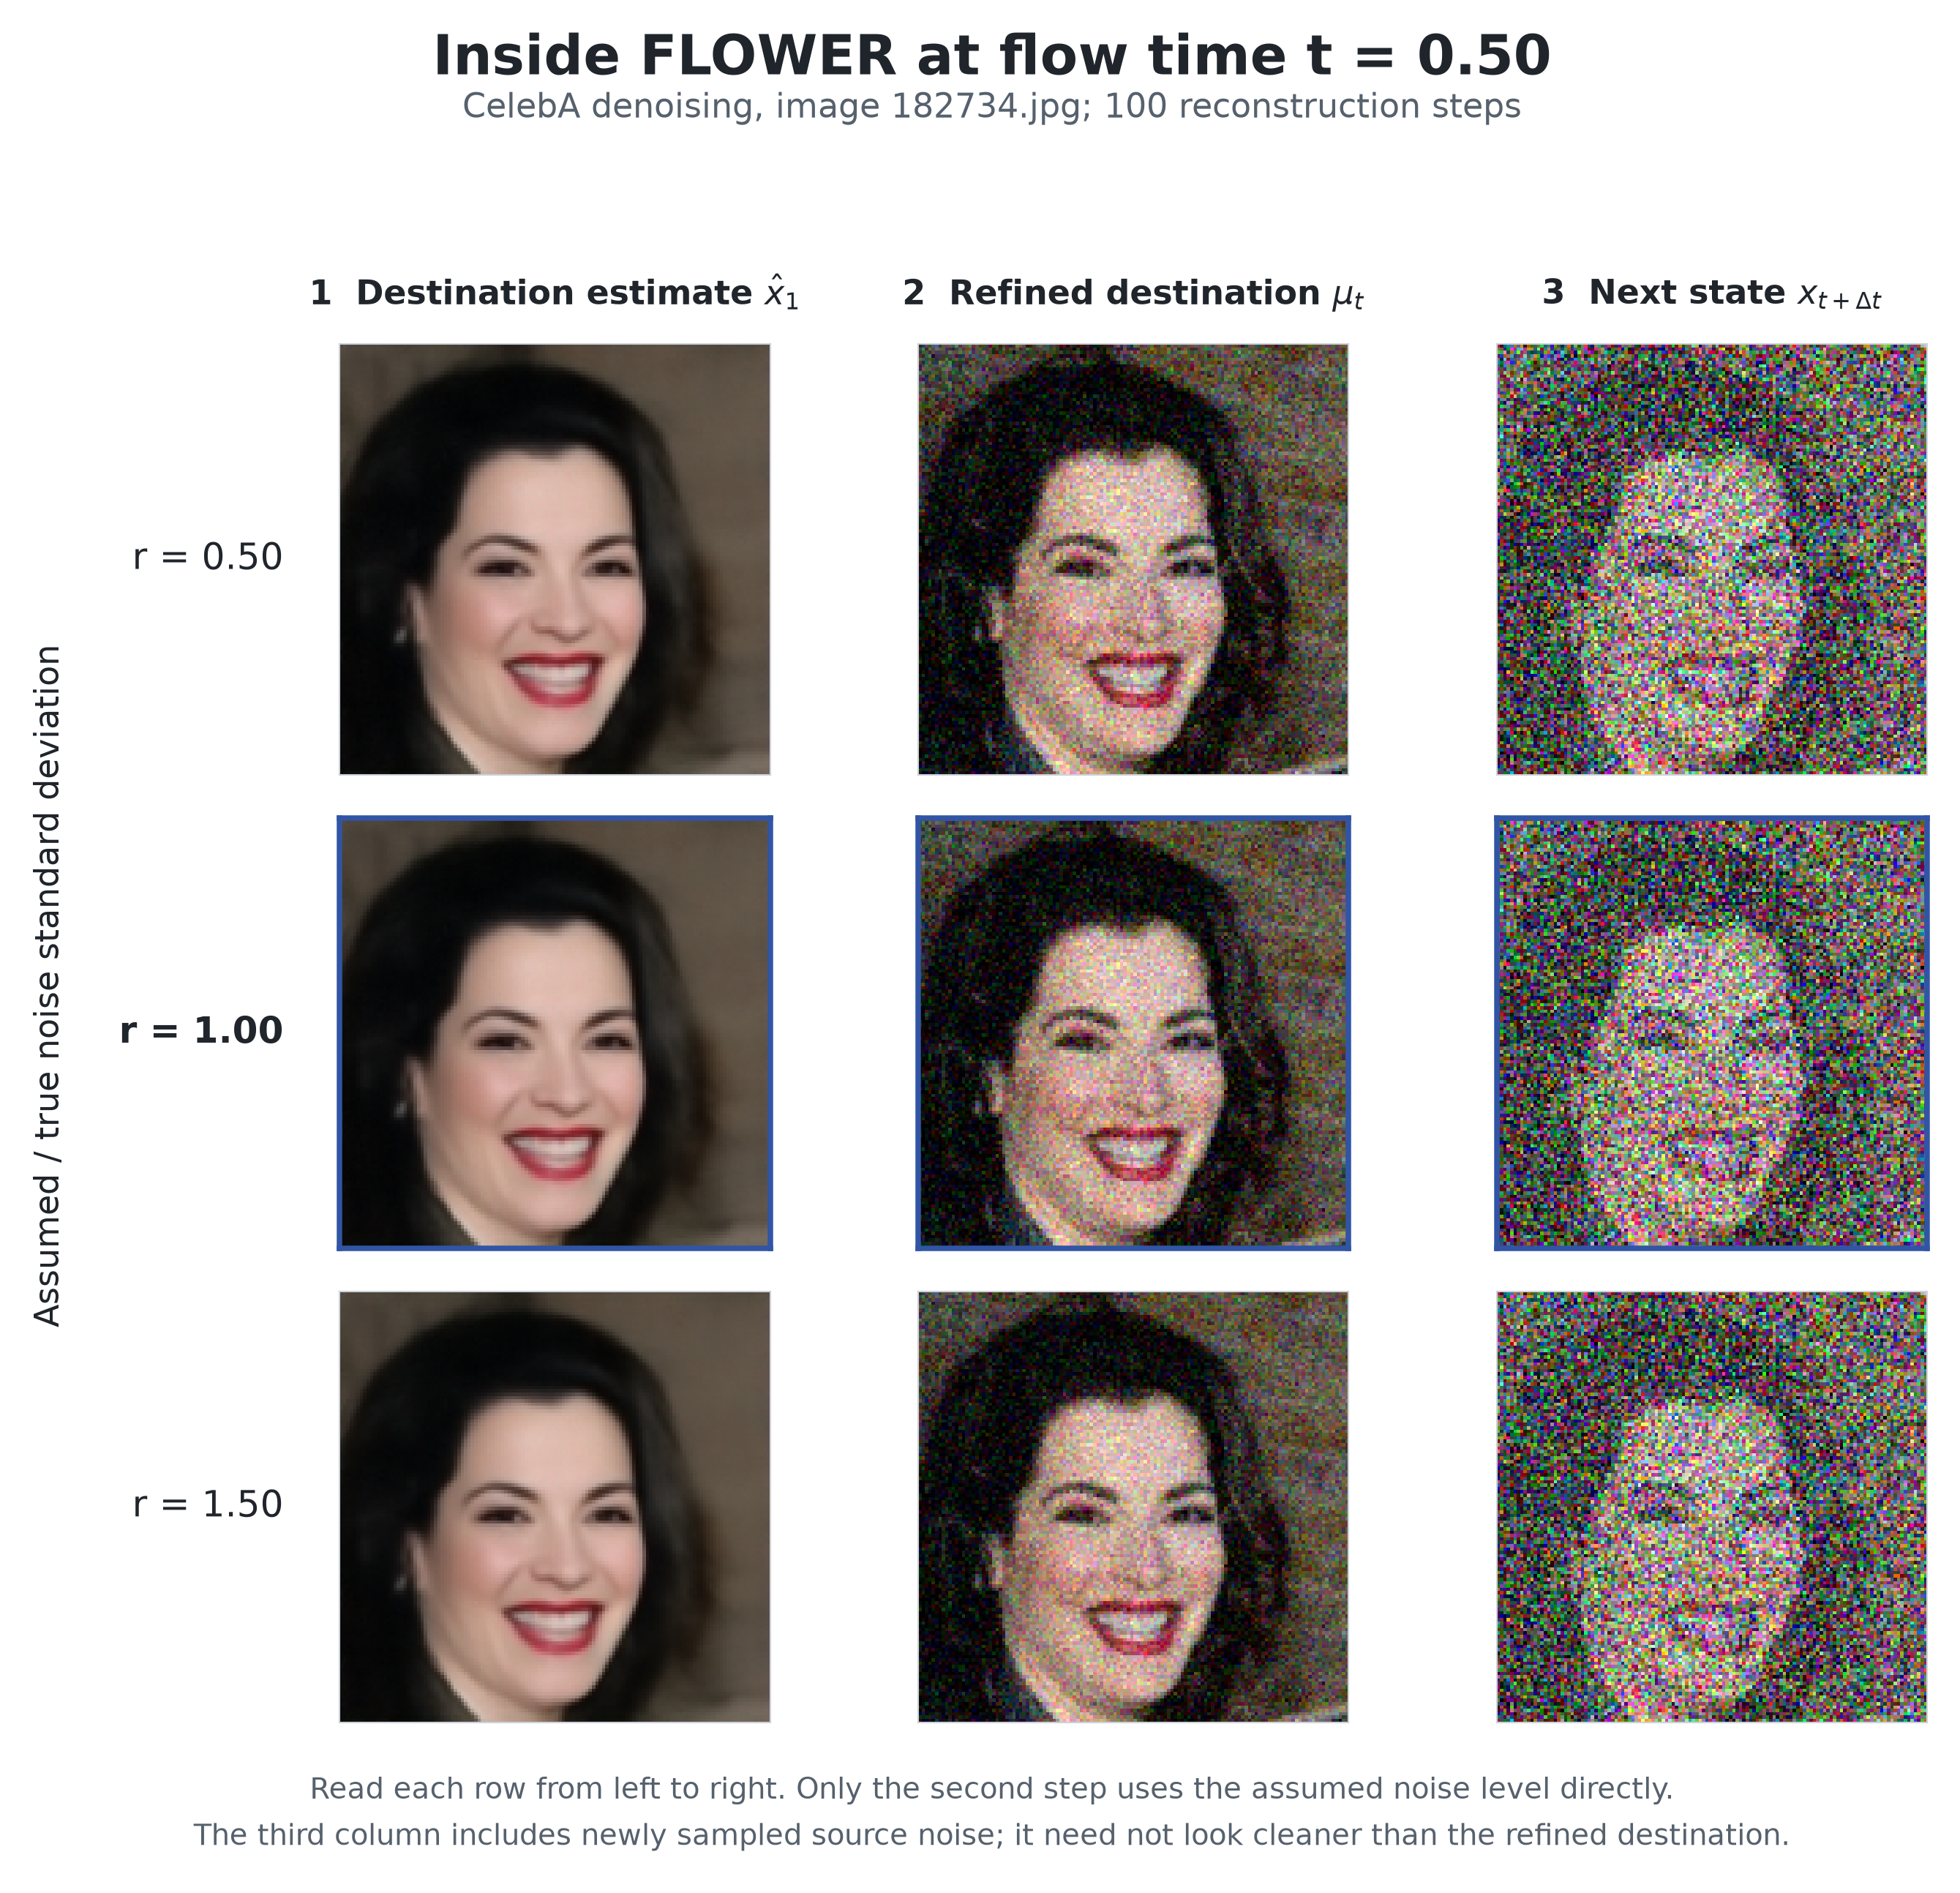
\includegraphics[width=.68\linewidth,height=.42\textheight,keepaspectratio]{10_internal_states_t05.png}

\caption{
Three internal FLOWER steps at $t=0.50$.
}

\label{fig:early050}

\end{figure}


% ============================================================
% APPENDIX E - ADDITIONAL METRIC FIGURES
% ============================================================

\section{Metric Comparisons by Inverse Problem}

These panels compare datasets for one inverse problem at a time.

Each metric uses its own vertical scale, making small differences
easier to distinguish than in the shared overview plots.

The numerical values and confidence intervals are the same
as those in Section 5.


\begin{figure}[htbp]

\centering

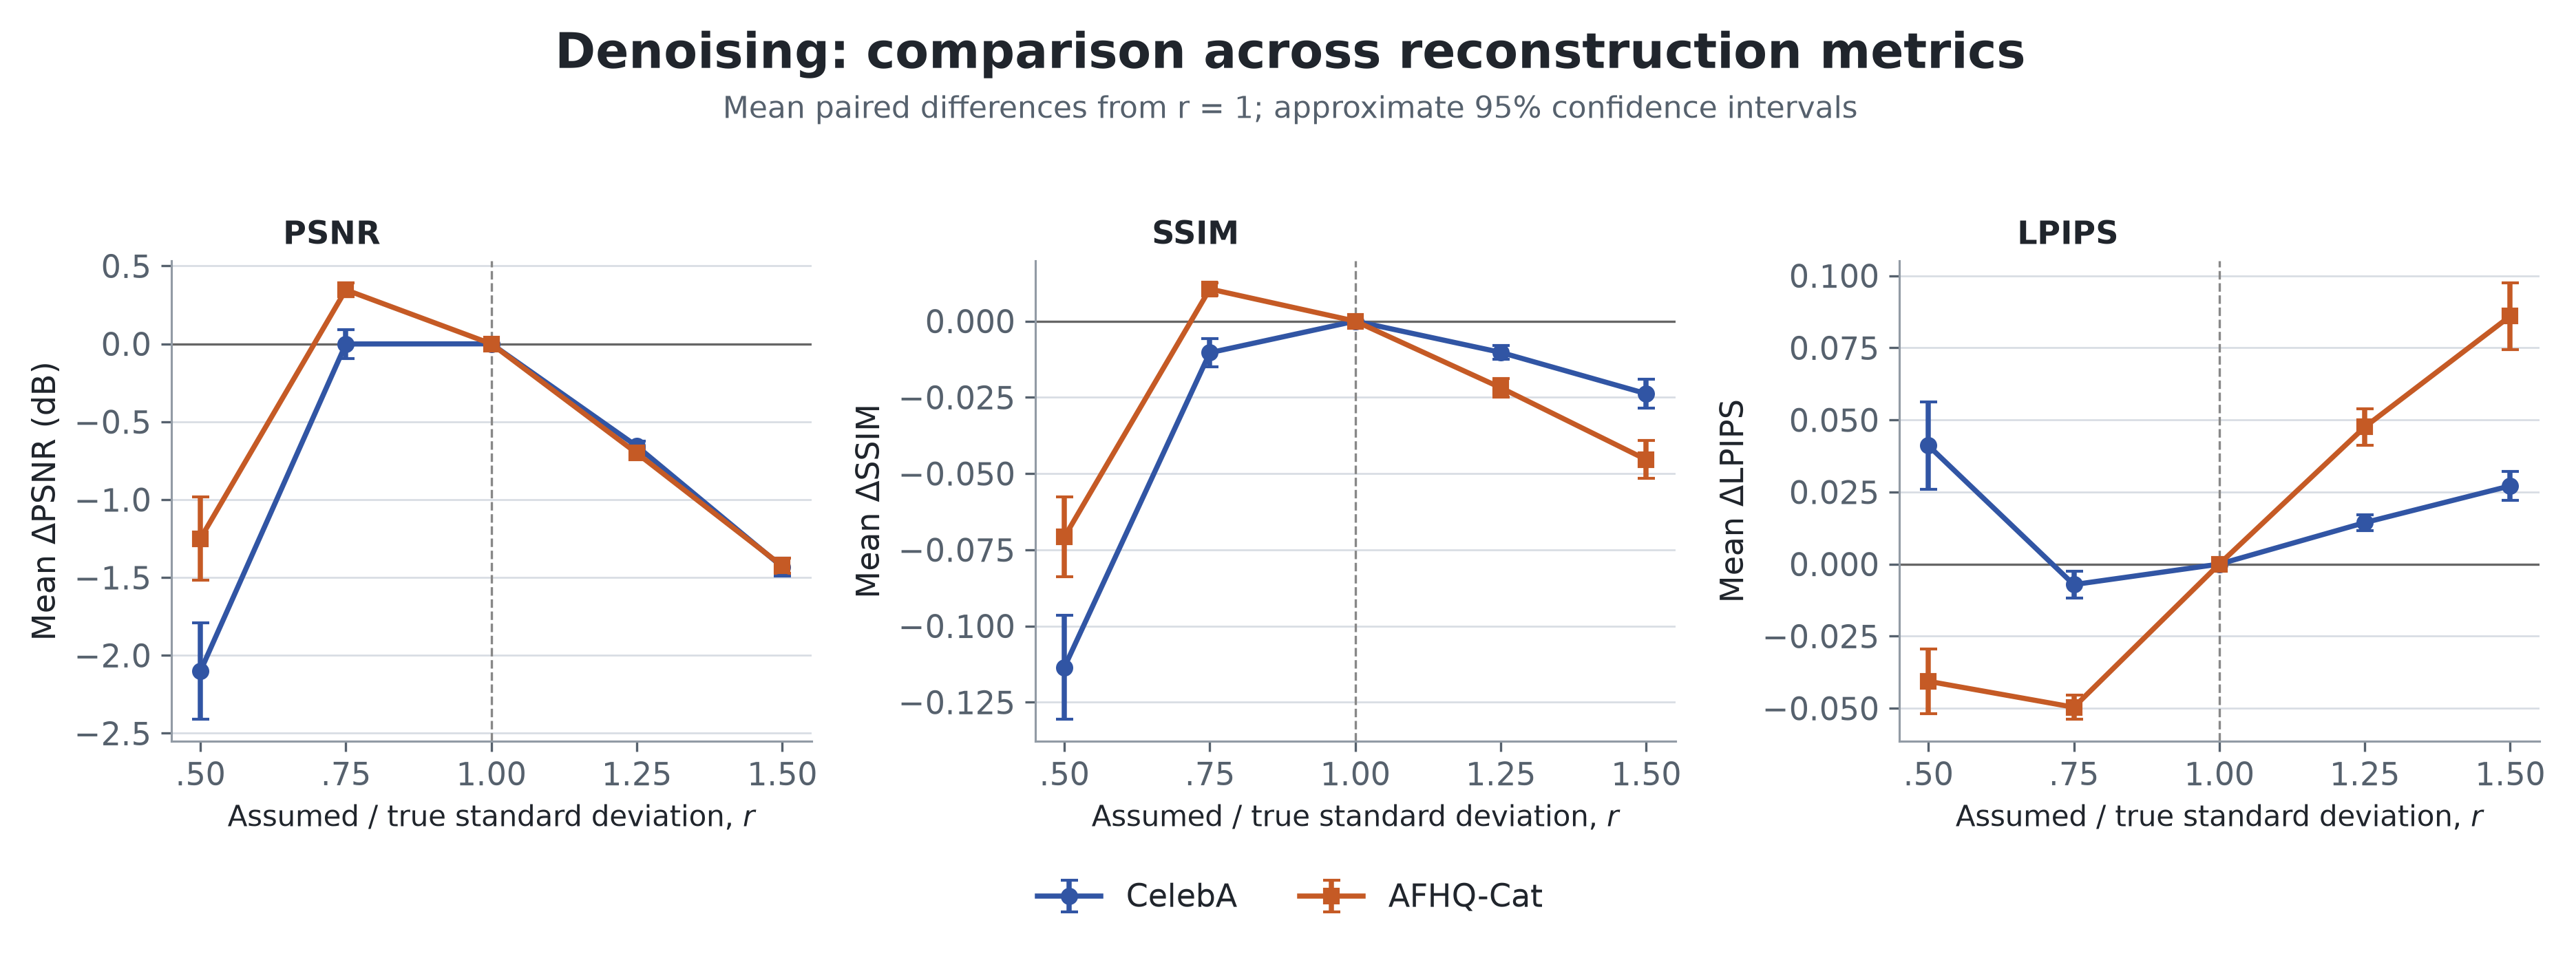
\includegraphics[width=\linewidth]{task_denoising.png}

\caption{
Denoising across PSNR, SSIM, and LPIPS.
AFHQ-Cat shows a perceptual--distortion trade-off at $r=0.5$.
}

\end{figure}


\begin{figure}[htbp]

\centering

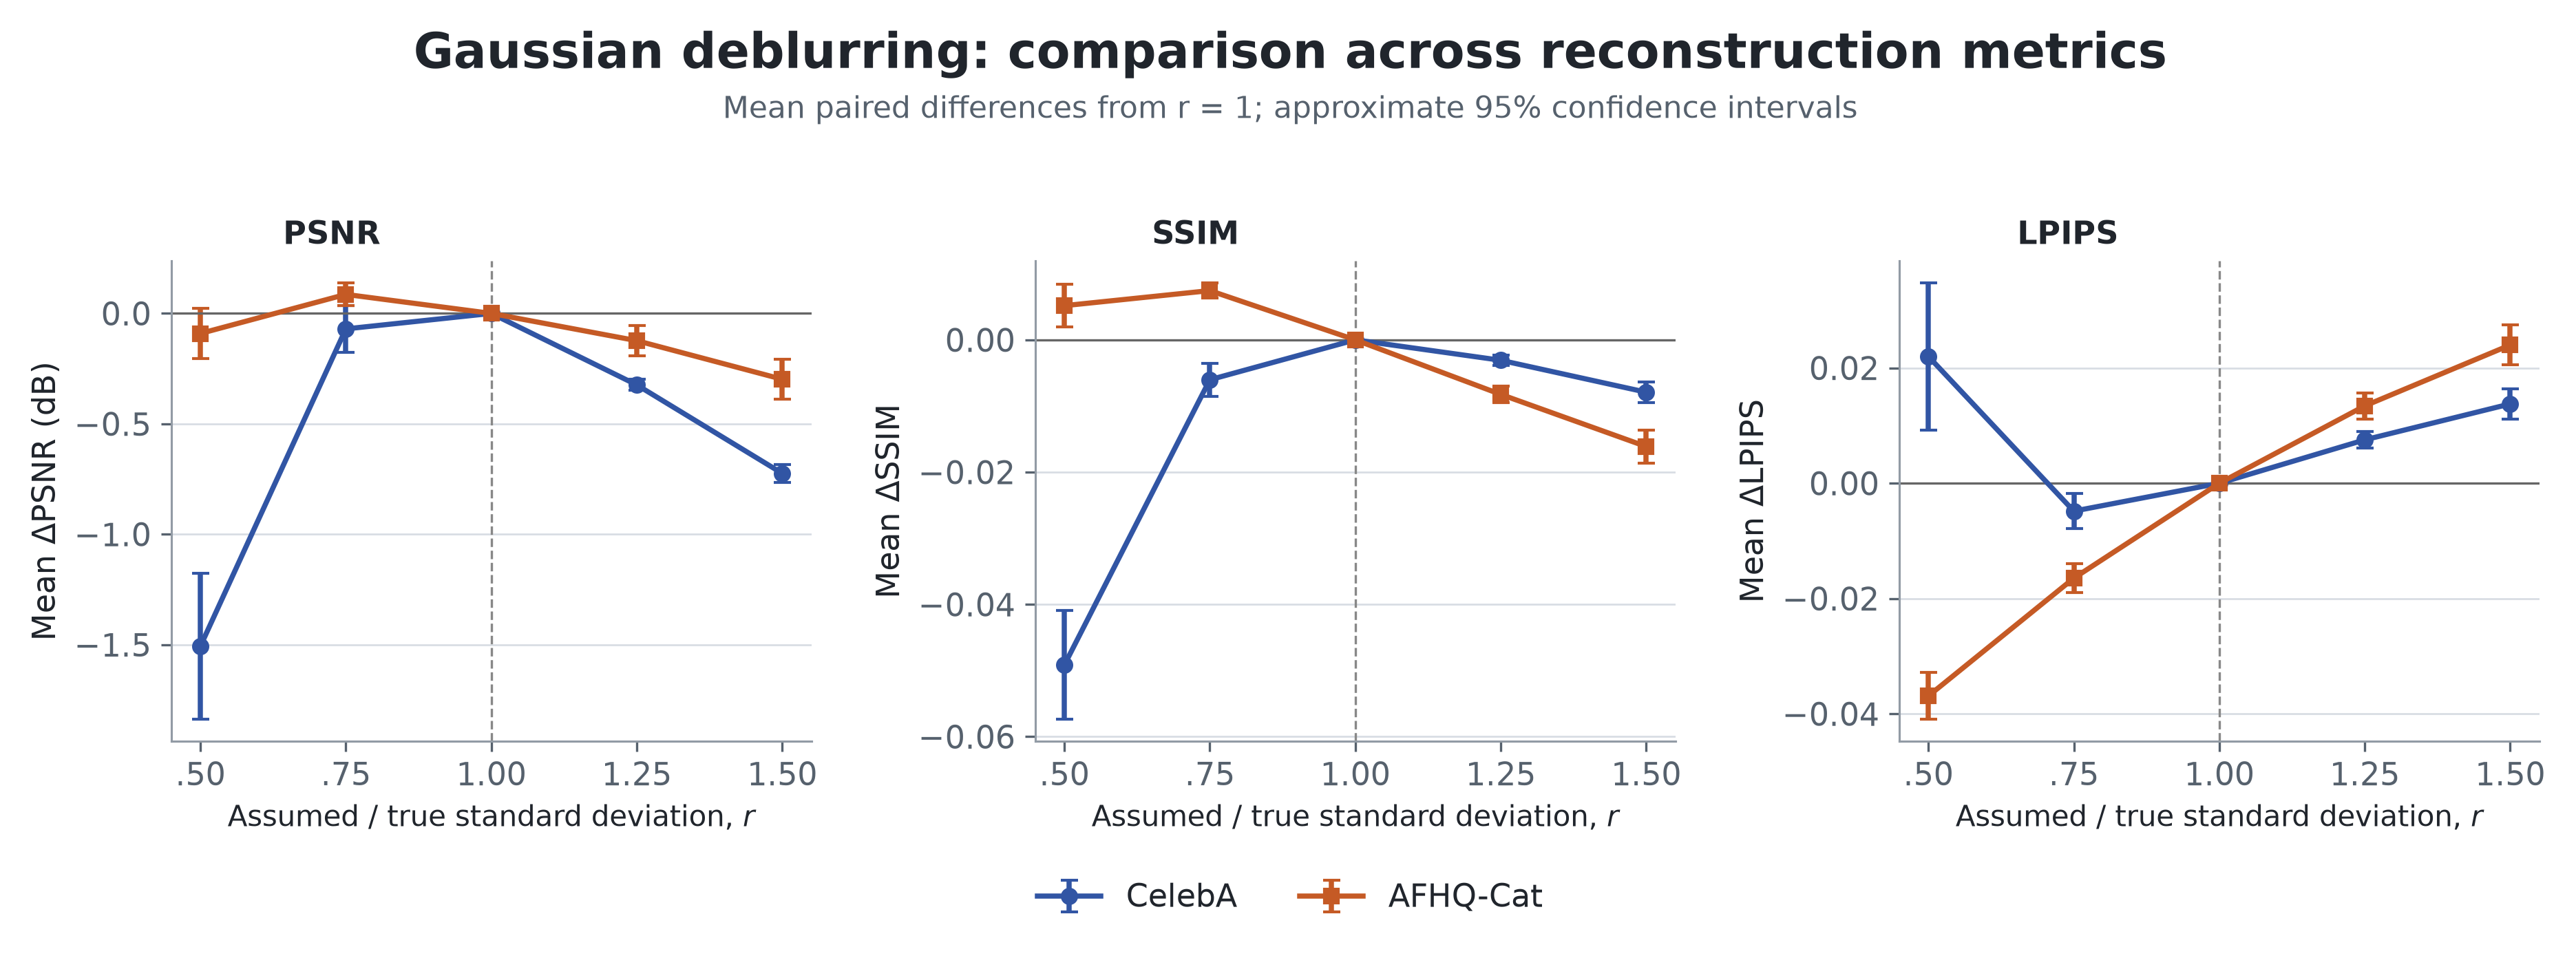
\includegraphics[width=\linewidth]{task_gaussian_deblurring.png}

\caption{
Gaussian deblurring across PSNR, SSIM, and LPIPS.
}

\end{figure}


\begin{figure}[htbp]

\centering

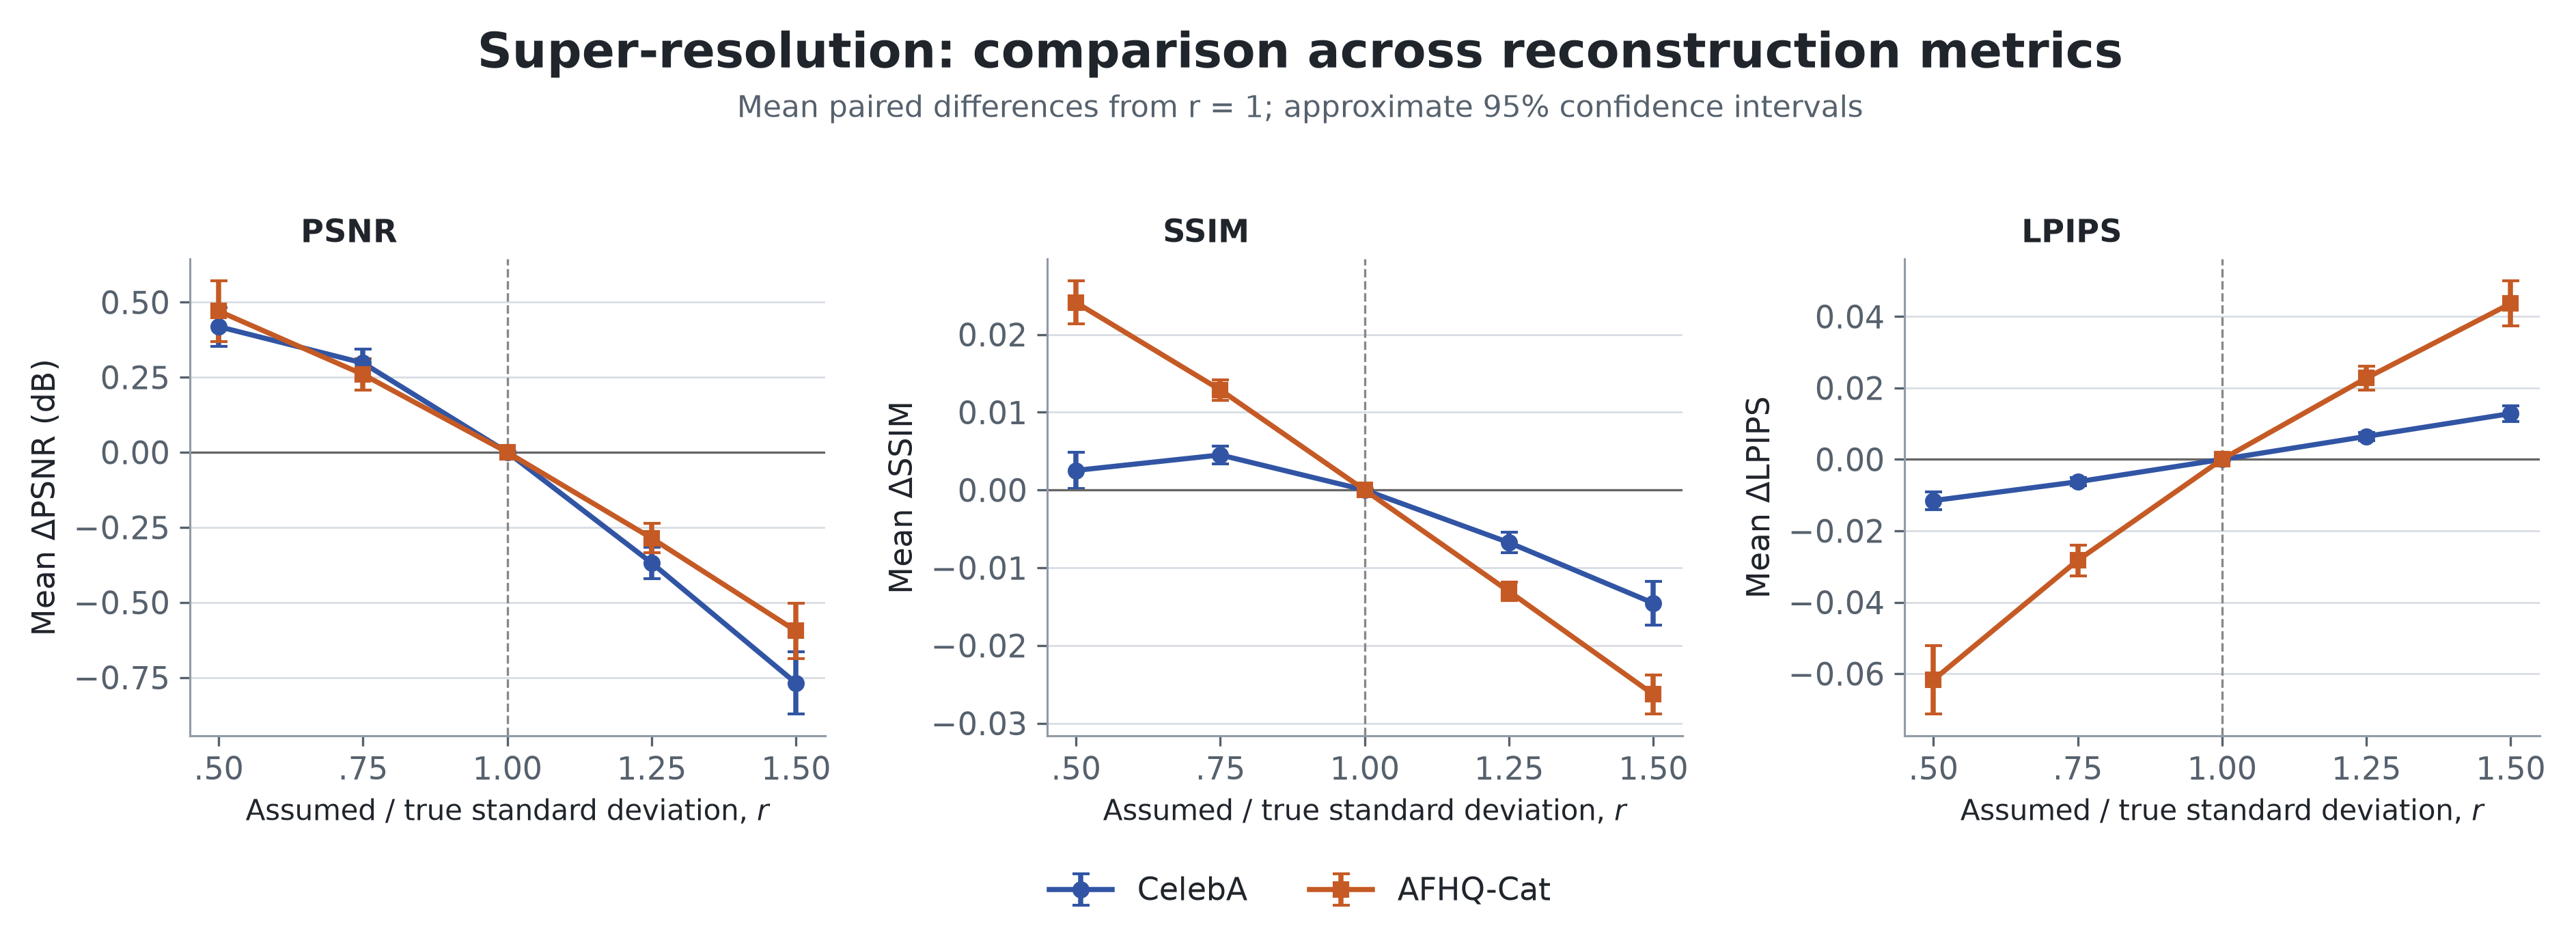
\includegraphics[width=\linewidth]{task_super_resolution.png}

\caption{
Super-resolution across PSNR, SSIM, and LPIPS.
All three metrics improve at $r=0.5$ on both datasets.
}

\end{figure}


\begin{figure}[htbp]

\centering

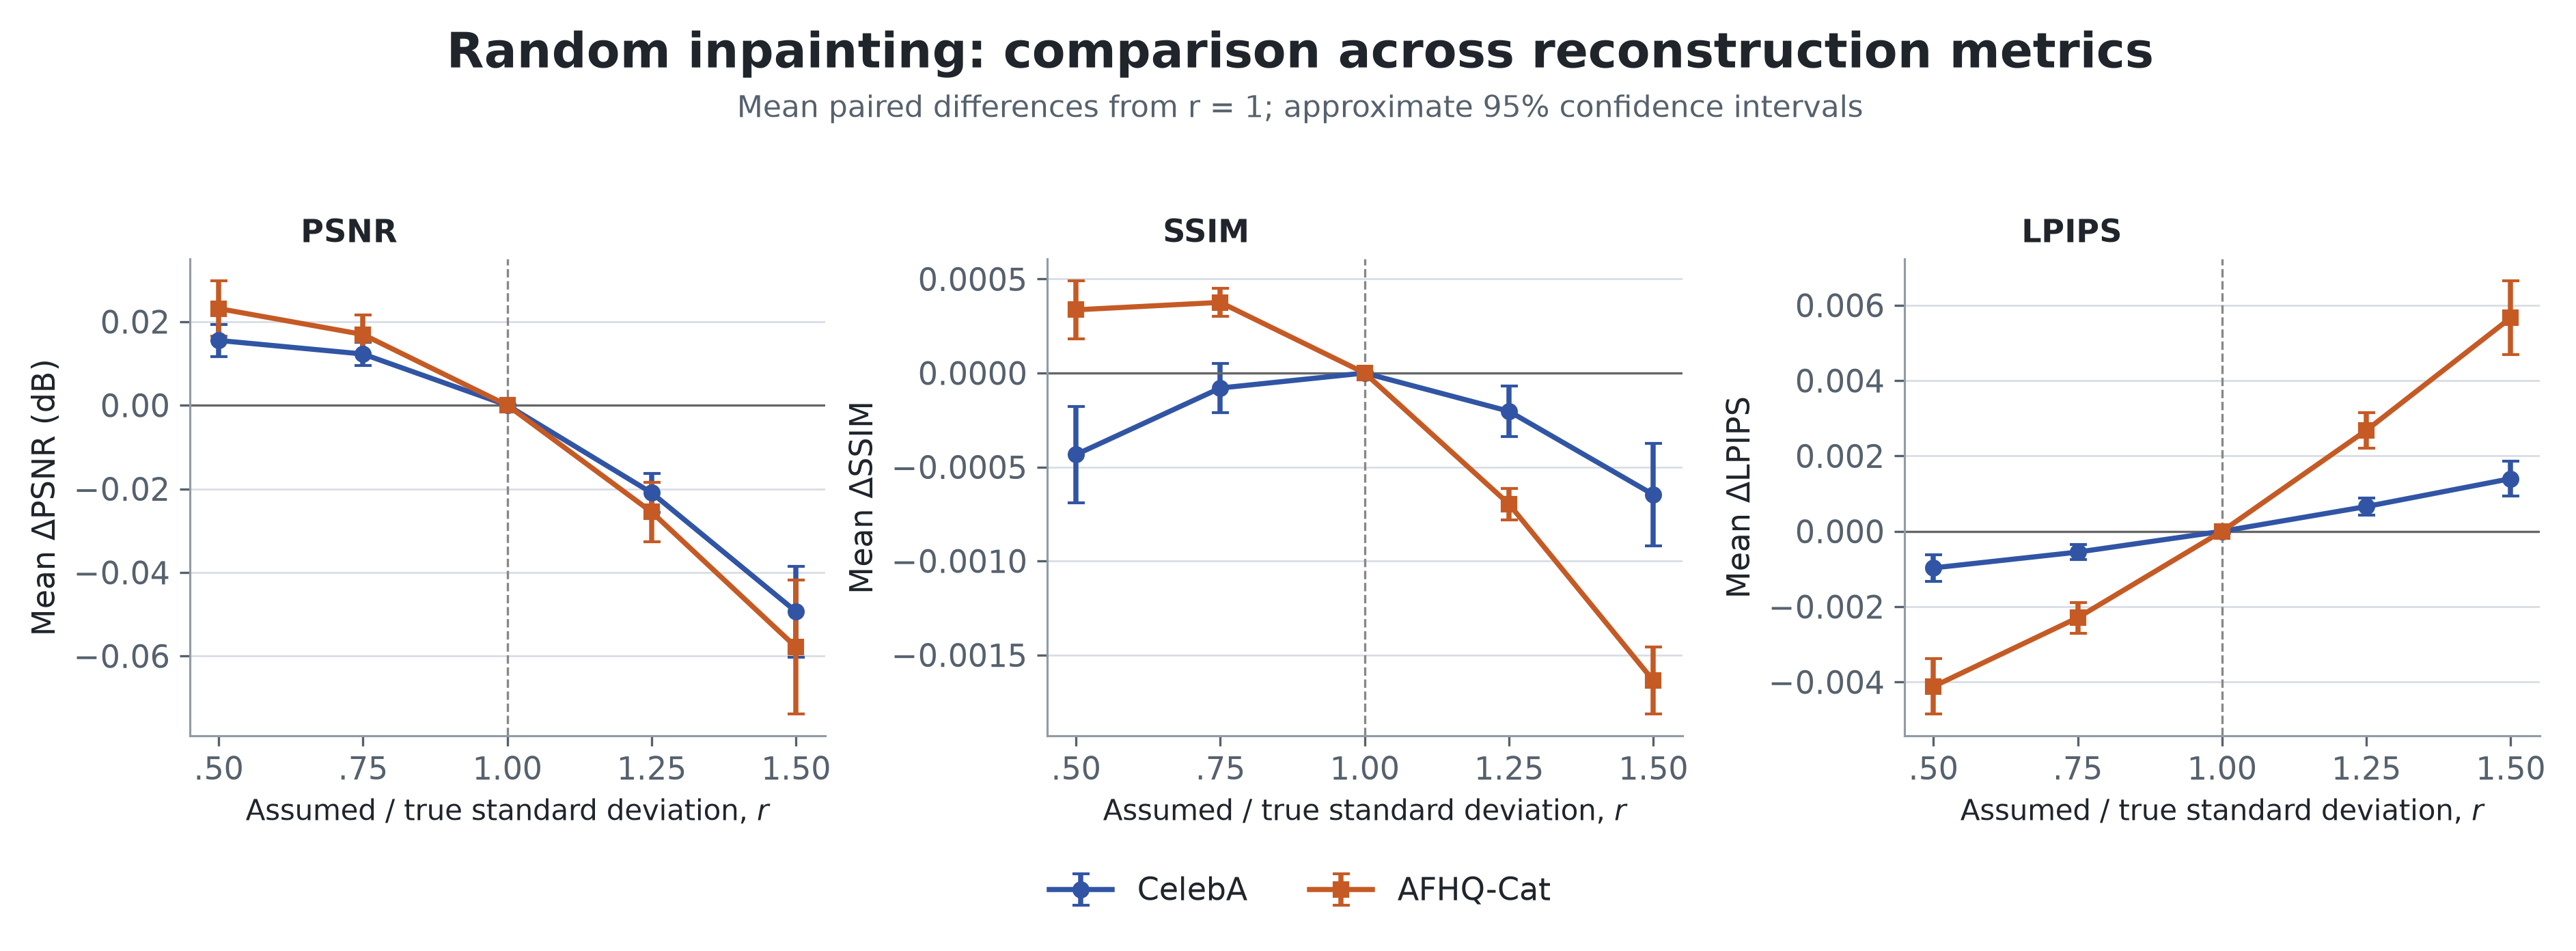
\includegraphics[width=\linewidth]{task_random_inpainting.png}

\caption{
Random inpainting across PSNR, SSIM, and LPIPS.
Changes are small in magnitude.
}

\end{figure}


\begin{figure}[htbp]

\centering

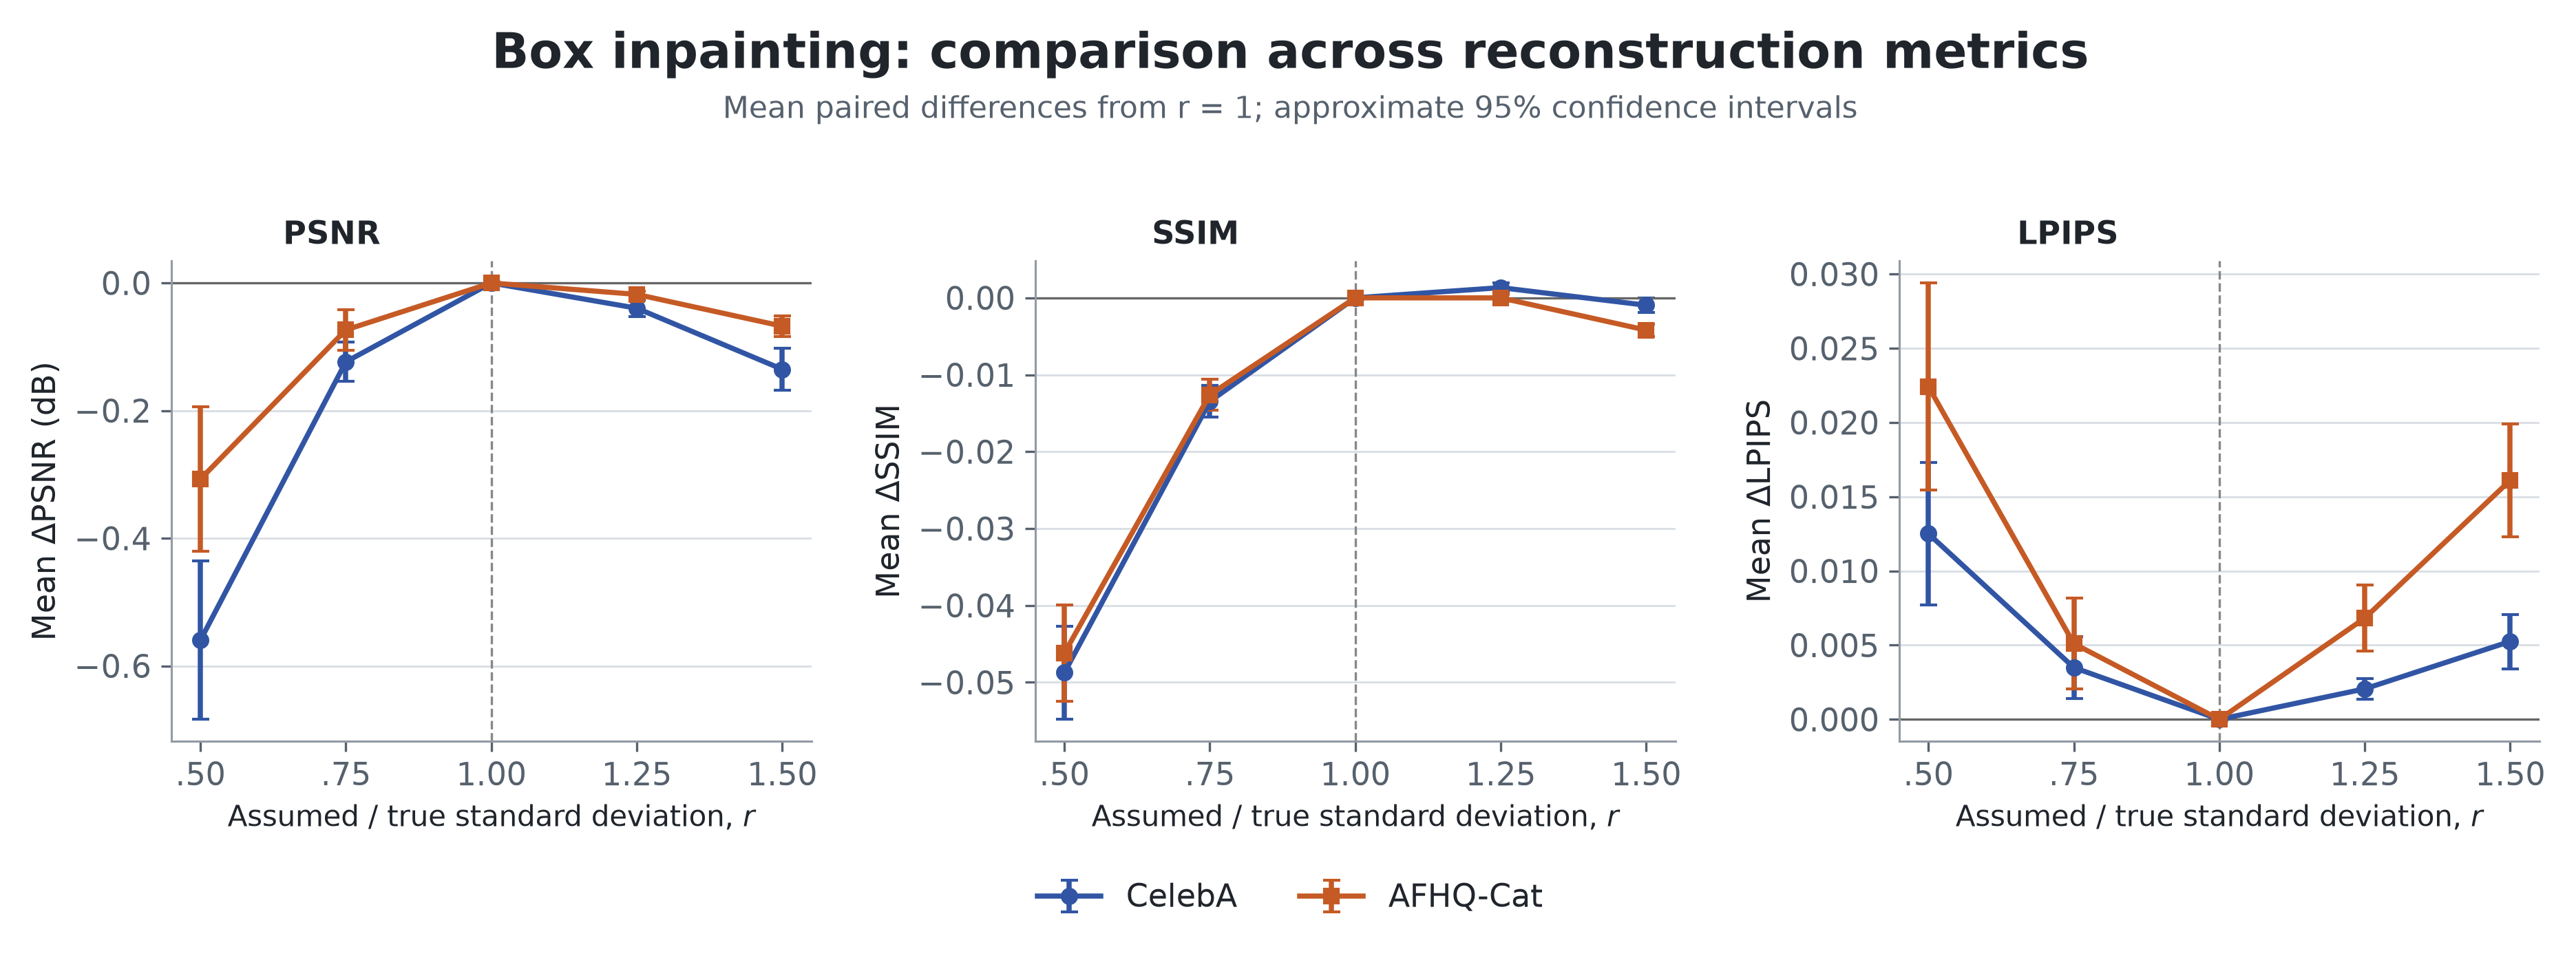
\includegraphics[width=\linewidth]{task_box_inpainting.png}

\caption{
Box inpainting across PSNR, SSIM, and LPIPS.
Underestimation can affect SSIM and LPIPS even where
PSNR changes are modest.
}

\end{figure}

\FloatBarrier


% ============================================================
% REFERENCES
% ============================================================

\begin{thebibliography}{9}

\bibitem{flower}

M. Pourya, B. El Rawas, and M. Unser.

\emph{FLOWER: A Flow-Matching Solver for Inverse Problems}.

ICLR, 2026.

\url{https://github.com/mehrsapo/Flower}.


\bibitem{lipman}

Y. Lipman, R. T. Q. Chen, H. Ben-Hamu, M. Nickel, and M. Le.

\emph{Flow Matching for Generative Modeling}.

ICLR, 2023.


\bibitem{pnpflow}

S. T. Martin, A. Gagneux, P. Hagemann, and G. Steidl.

\emph{PnP-Flow: Plug-and-Play Image Restoration with Flow Matching}.

ICLR, 2025.


\end{thebibliography}

\end{document}
